\section{\zpsel pre-selection}
\label{app:nuepresel}

Figures~\ref{fig:1e0p:dataMCRun1:reco_nu_vtx}-\ref{fig:1e0p:dataMCRun1:shrlen} show the data-MC comparison for all \zpsel variables in run 1 and run 3 open data after \zpsel pre-selection.

\begin{figure}[H] 
\begin{center}
    \begin{subfigure}[b]{0.3\textwidth}
    \centering
    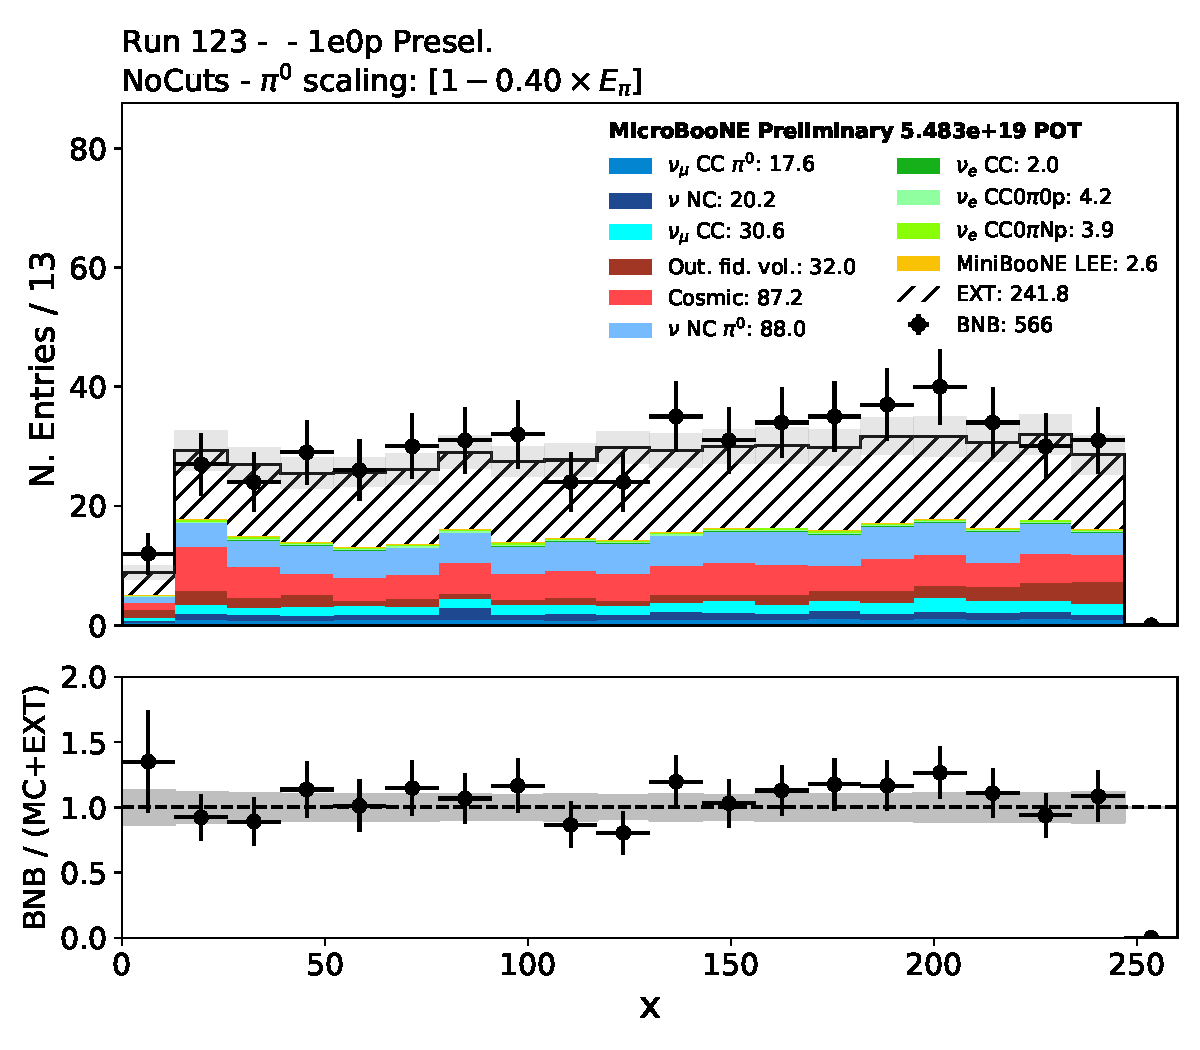
\includegraphics[width=1.00\textwidth]{1e0p/dataMCRun123/reco_nu_vtx_x.pdf}
    \caption{\label{fig:1e0p:dataMCRun1:reco_nu_vtx_x} reco\_nu\_vtx\_x }
    \end{subfigure}
    \begin{subfigure}[b]{0.3\textwidth}
    \centering
    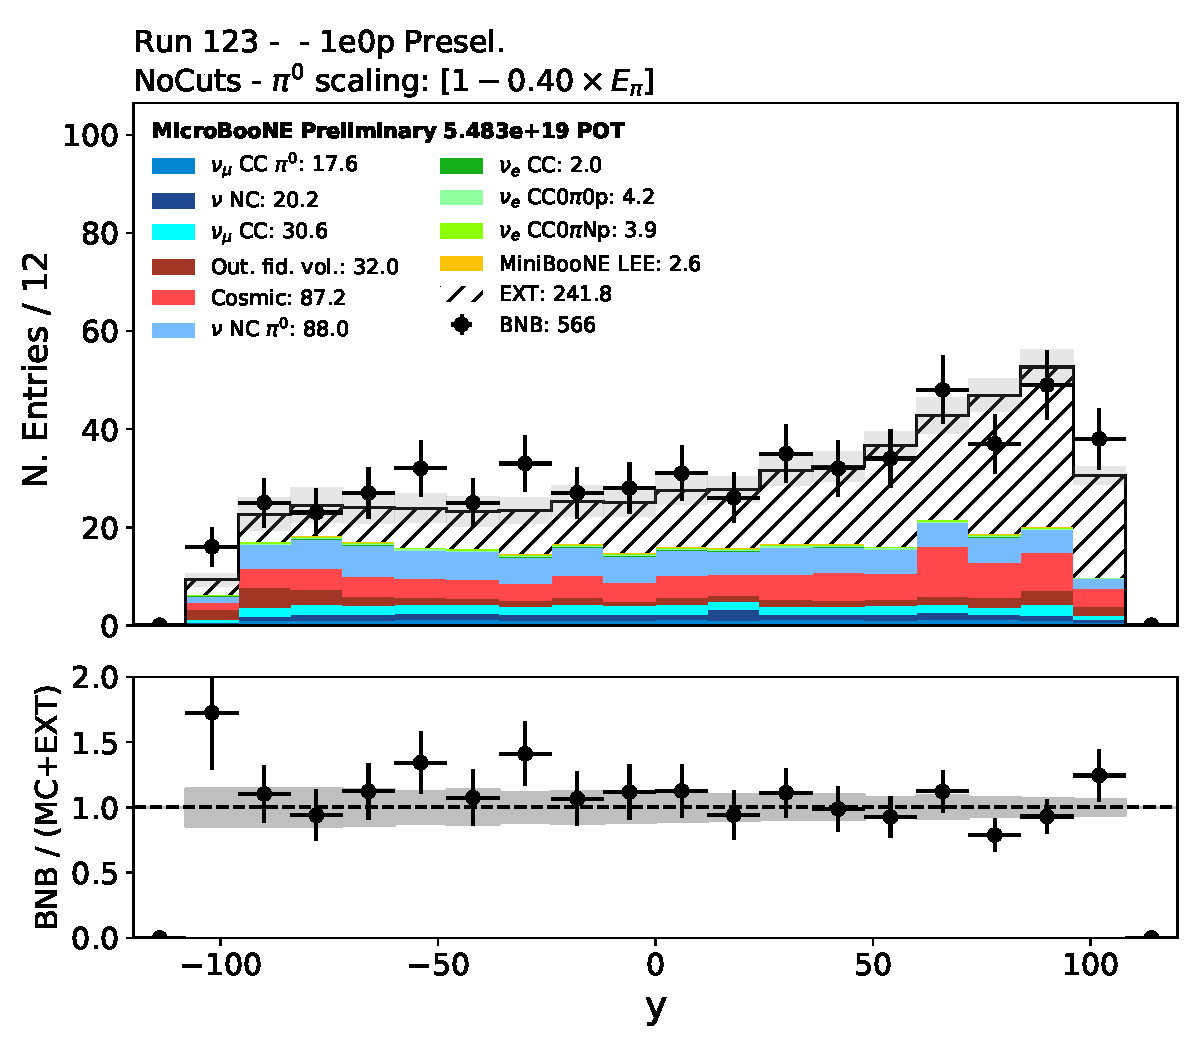
\includegraphics[width=1.00\textwidth]{1e0p/dataMCRun123/reco_nu_vtx_y.pdf}
    \caption{\label{fig:1e0p:dataMCRun1:reco_nu_vtx_y} reco\_nu\_vtx\_y}
    \end{subfigure}
    \begin{subfigure}[b]{0.3\textwidth}
    \centering
    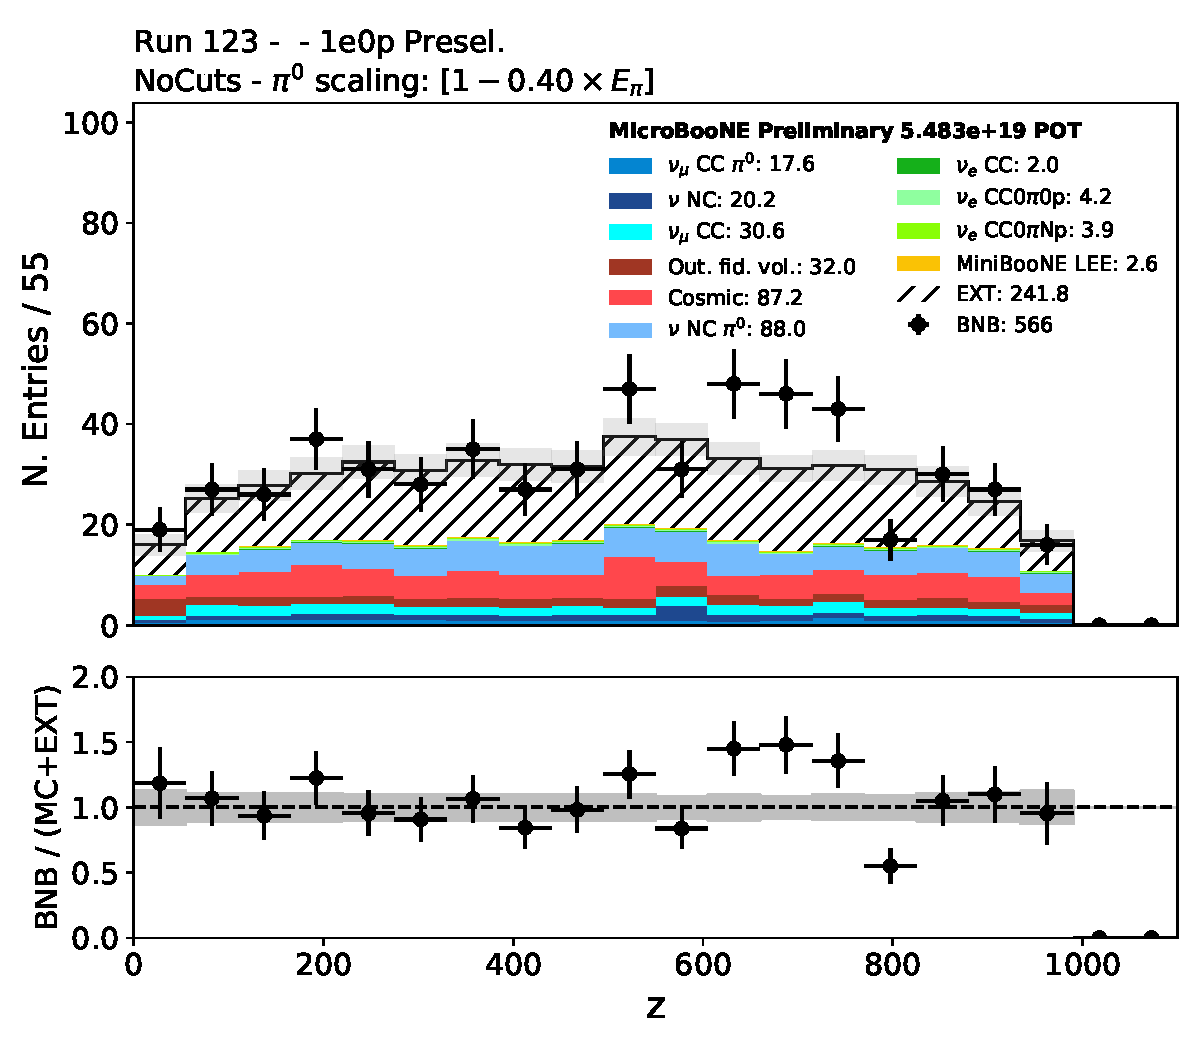
\includegraphics[width=1.00\textwidth]{1e0p/dataMCRun123/reco_nu_vtx_z.pdf}
    \caption{\label{fig:1e0p:dataMCRun1:reco_nu_vtx_z} reco\_nu\_vtx\_z}
    \end{subfigure}
\caption{\label{fig:1e0p:dataMCRun1:reco_nu_vtx}Data-MC comparison in the open data after the \zpsel pre-selection.}
\end{center}
\end{figure}

\begin{figure}[H] 
\begin{center}
    \begin{subfigure}[b]{0.3\textwidth}
    \centering
    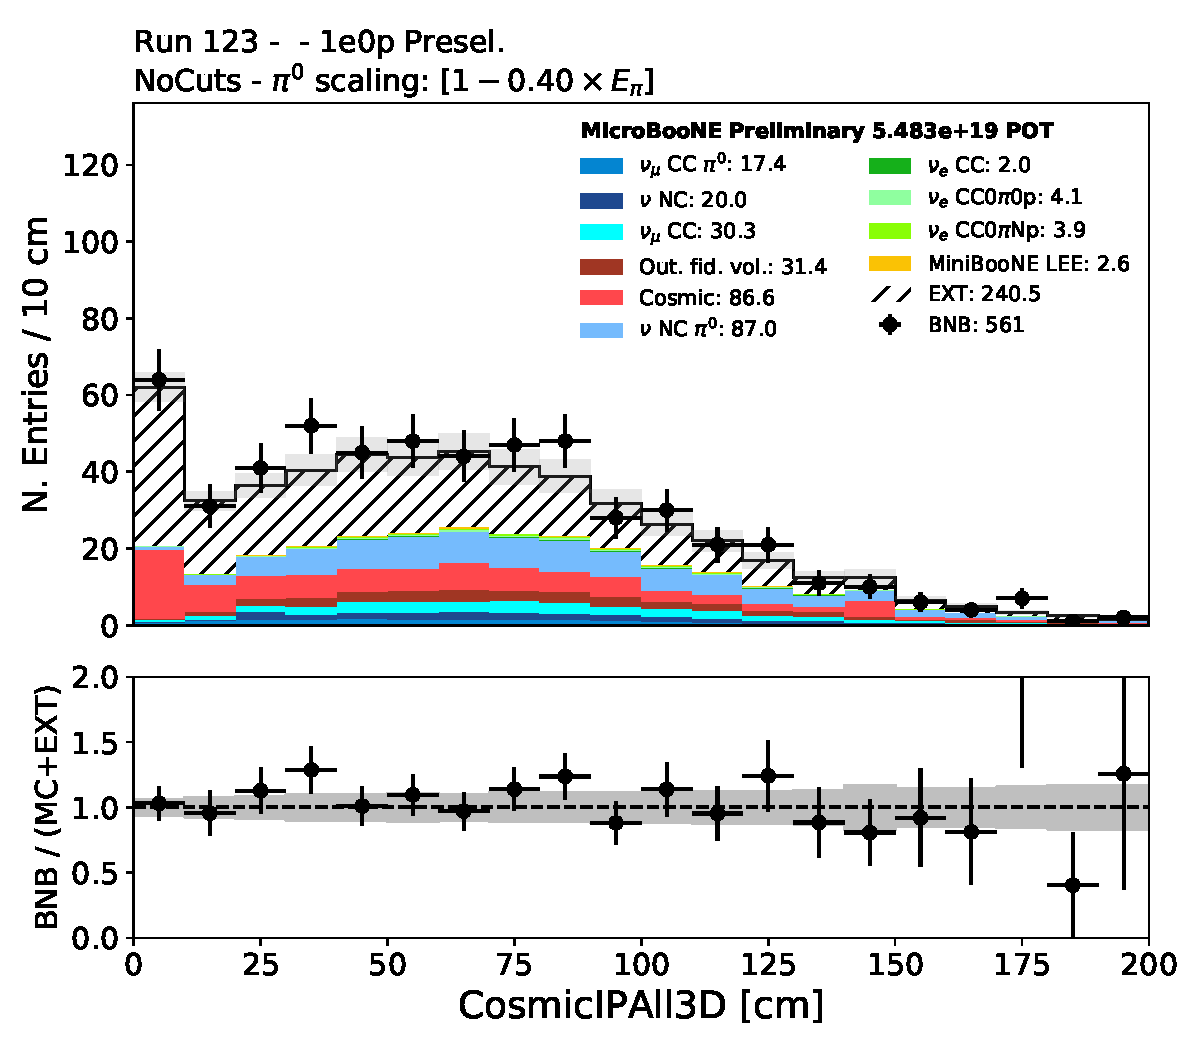
\includegraphics[width=1.00\textwidth]{1e0p/dataMCRun123/CosmicIPAll3D.pdf}
    \caption{\label{fig:1e0p:dataMCRun1:CosmicIP} CosmicIP3D }
    \end{subfigure}
    \begin{subfigure}[b]{0.3\textwidth}
    \centering
    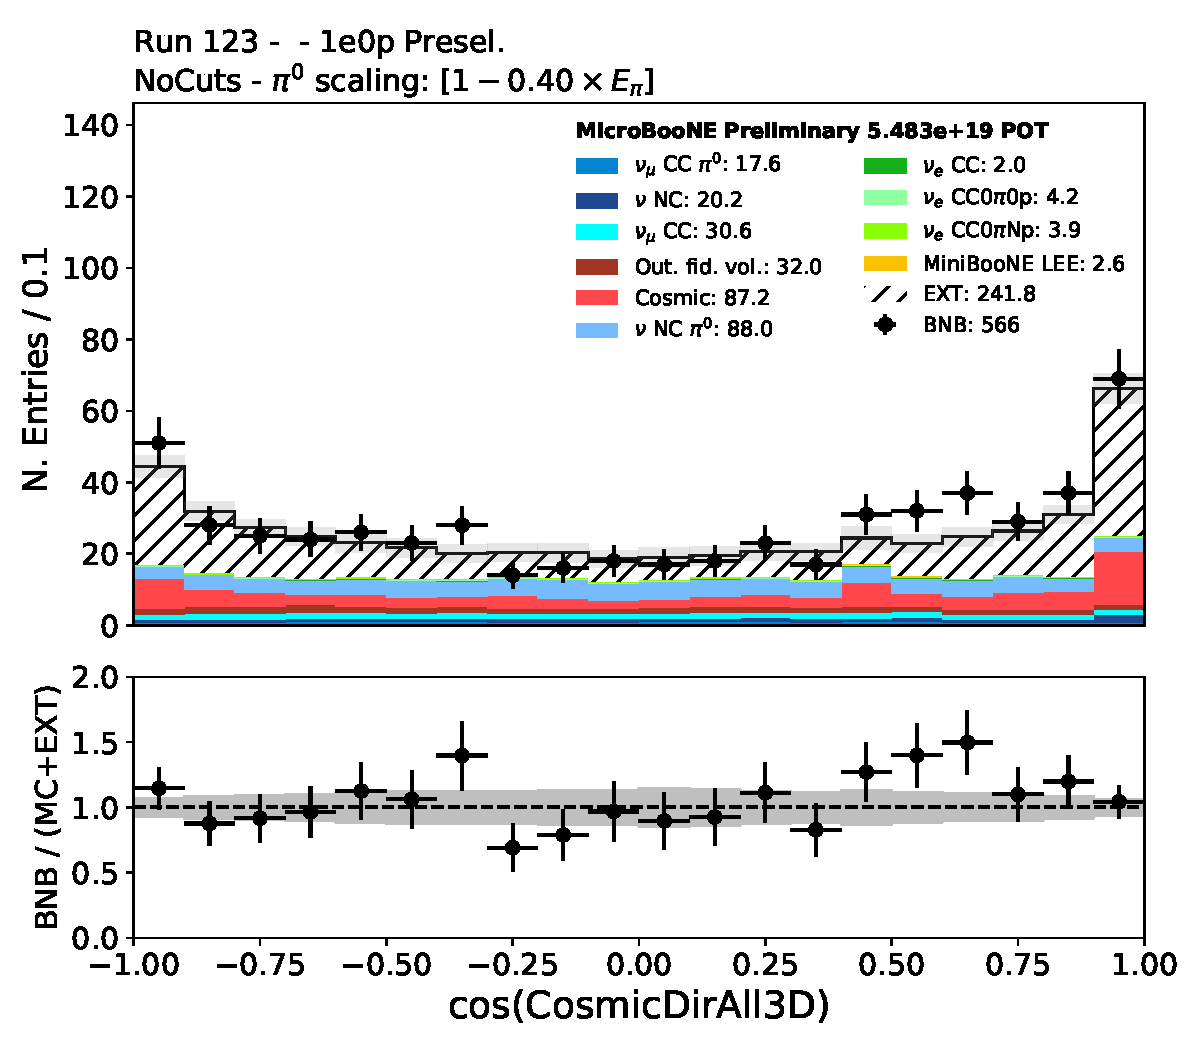
\includegraphics[width=1.00\textwidth]{1e0p/dataMCRun123/CosmicDirAll3D.pdf}
    \caption{\label{fig:1e0p:dataMCRun1:CosmicIP} CosmicDir3D }
    \end{subfigure}
    \begin{subfigure}[b]{0.3\textwidth}
    \centering
    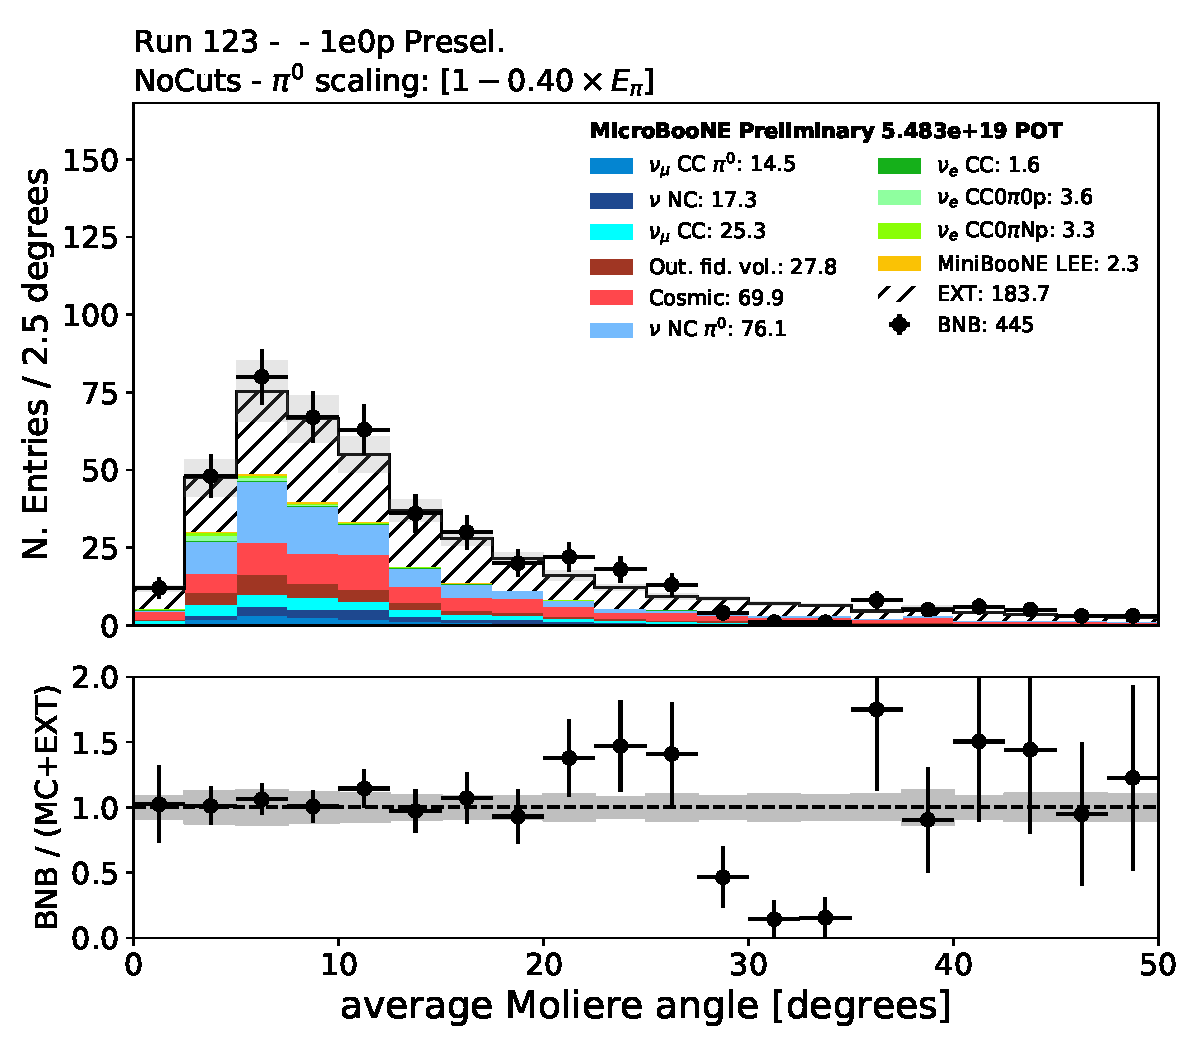
\includegraphics[width=1.00\textwidth]{1e0p/dataMCRun123/shrmoliereavg.pdf}
    \caption{\label{fig:1e0p:dataMCRun1:shrmoliereavg} shrmoliereavg }
    \end{subfigure}
\caption{\label{fig:1e0p:dataMCRun1:cosmic}Data-MC comparison in the open data after the \zpsel preselection.}
\end{center}
\end{figure}

\begin{figure}[H] 
\begin{center}
    \begin{subfigure}[b]{0.3\textwidth}
    \centering
    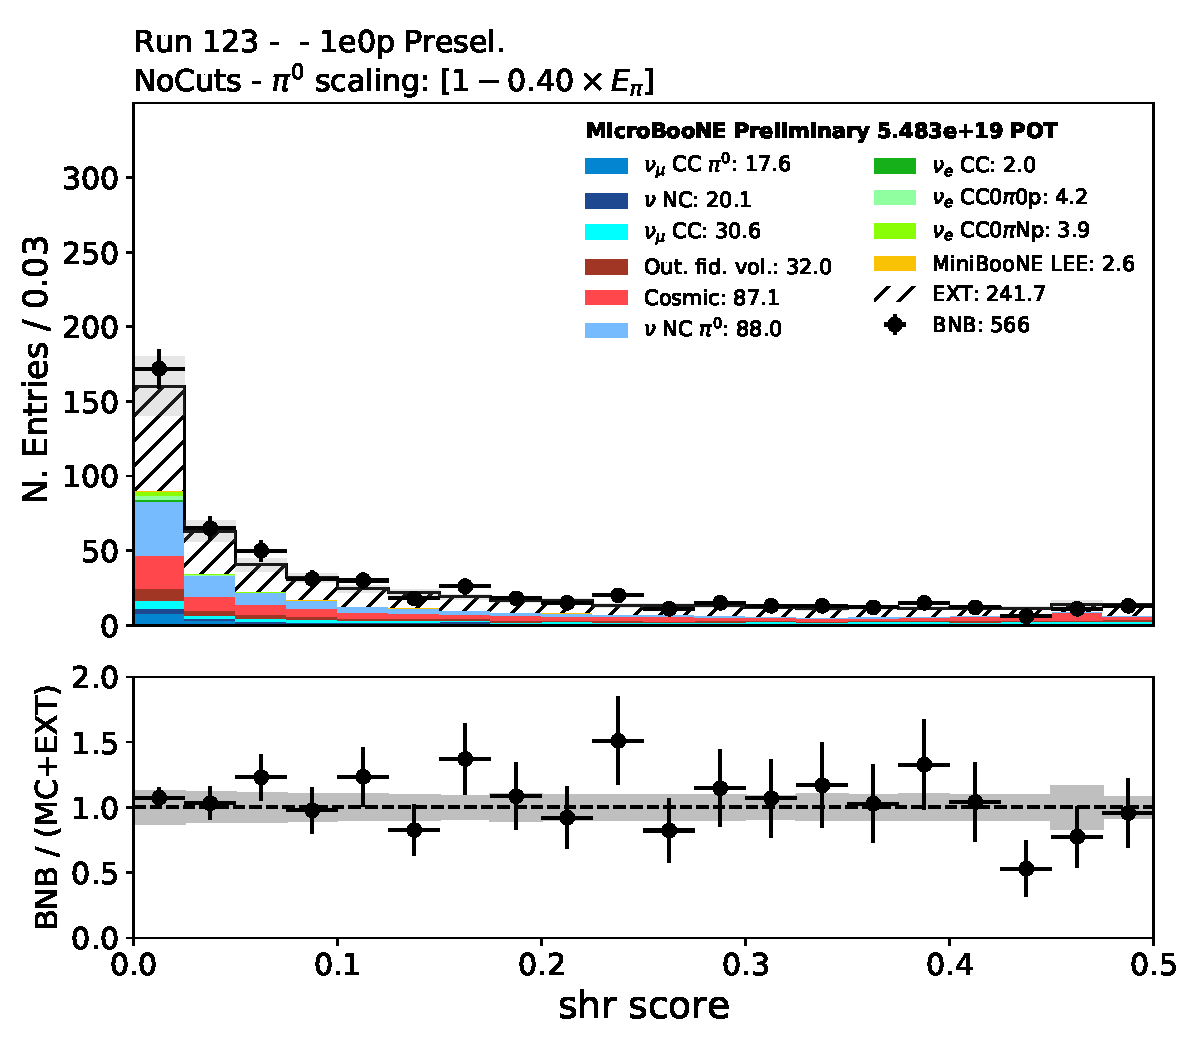
\includegraphics[width=1.00\textwidth]{1e0p/dataMCRun123/shr_score.pdf}
    \caption{\label{fig:1e0p:dataMCRun1:shr_score} shr\_score }
    \end{subfigure}
    \begin{subfigure}[b]{0.3\textwidth}
    \centering
    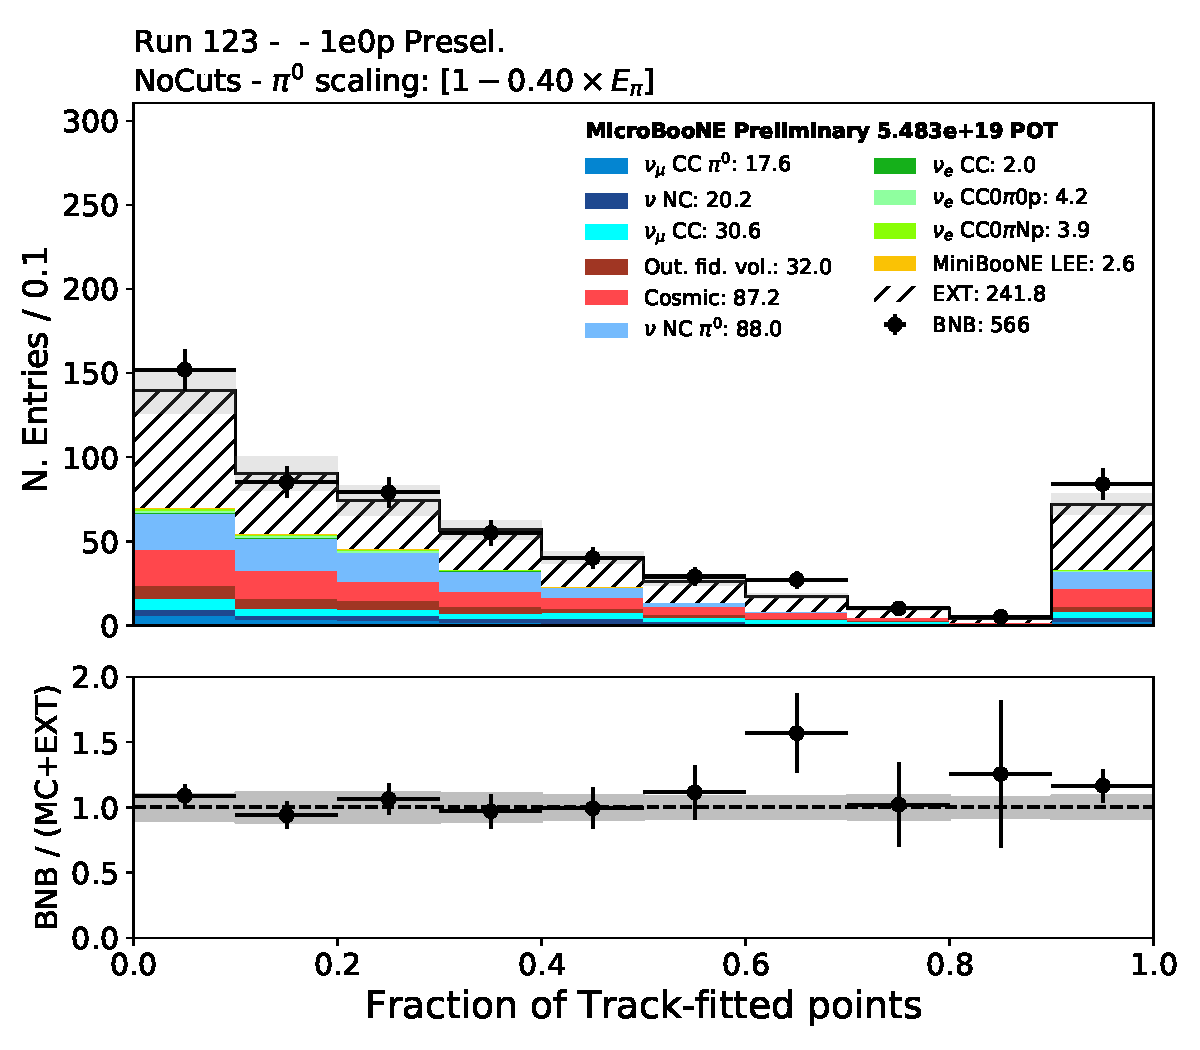
\includegraphics[width=1.00\textwidth]{1e0p/dataMCRun123/trkfit.pdf}
    \caption{\label{fig:1e0p:dataMCRun1:trkfit} trkfit }
    \end{subfigure}
    \begin{subfigure}[b]{0.3\textwidth}
    \centering
    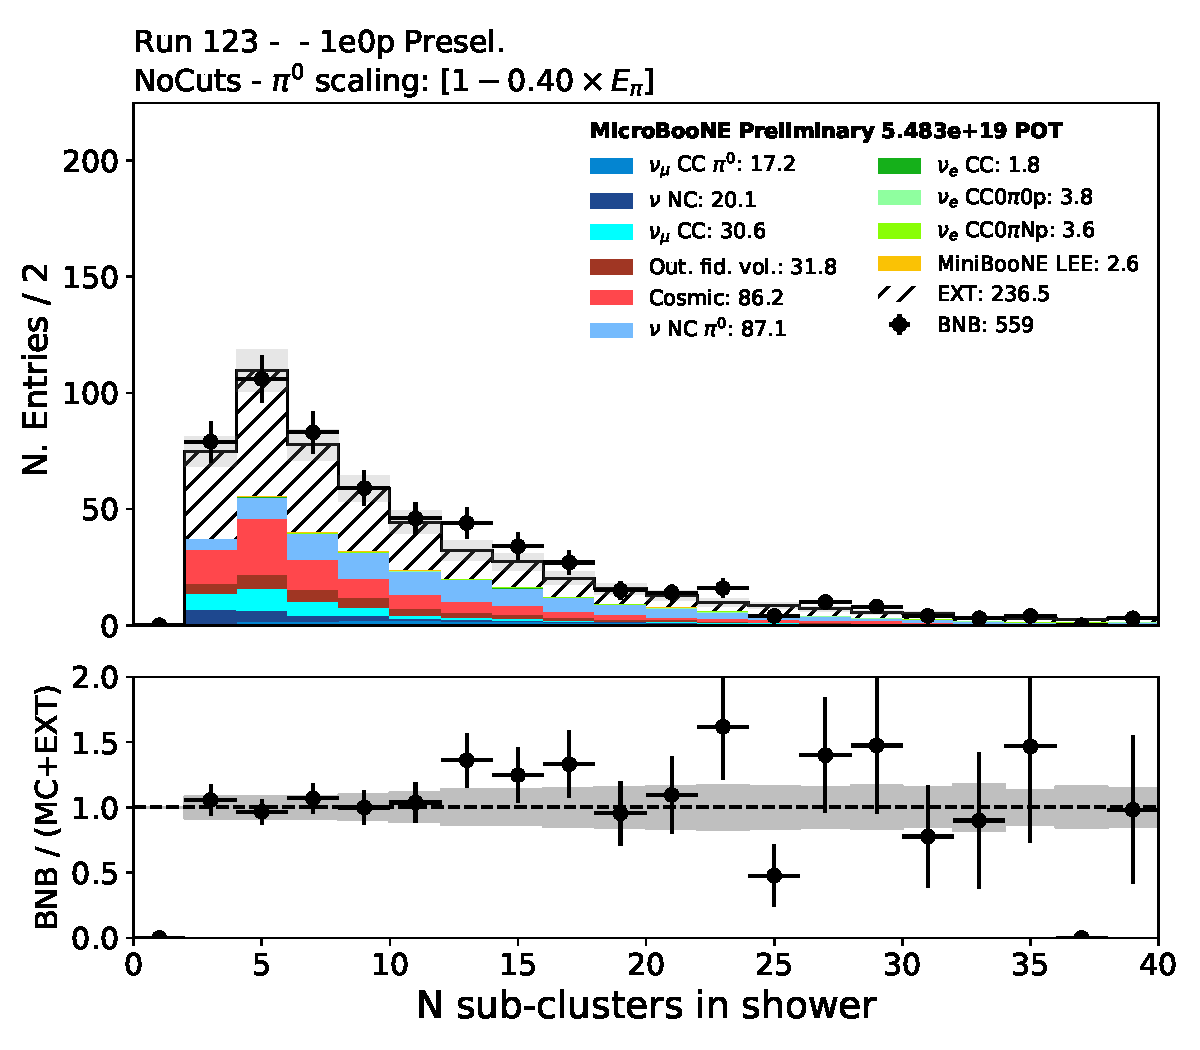
\includegraphics[width=1.00\textwidth]{1e0p/dataMCRun123/subcluster.pdf}
    \caption{\label{fig:1e0p:dataMCRun1:subcluster} subcluster }
    \end{subfigure}
\caption{\label{fig:1e0p:dataMCRun1:numu1}Data-MC comparison in the open data after the \zpsel preselection.}
\end{center}
\end{figure}

\begin{figure}[H] 
\begin{center}
    \begin{subfigure}[b]{0.3\textwidth}
    \centering
    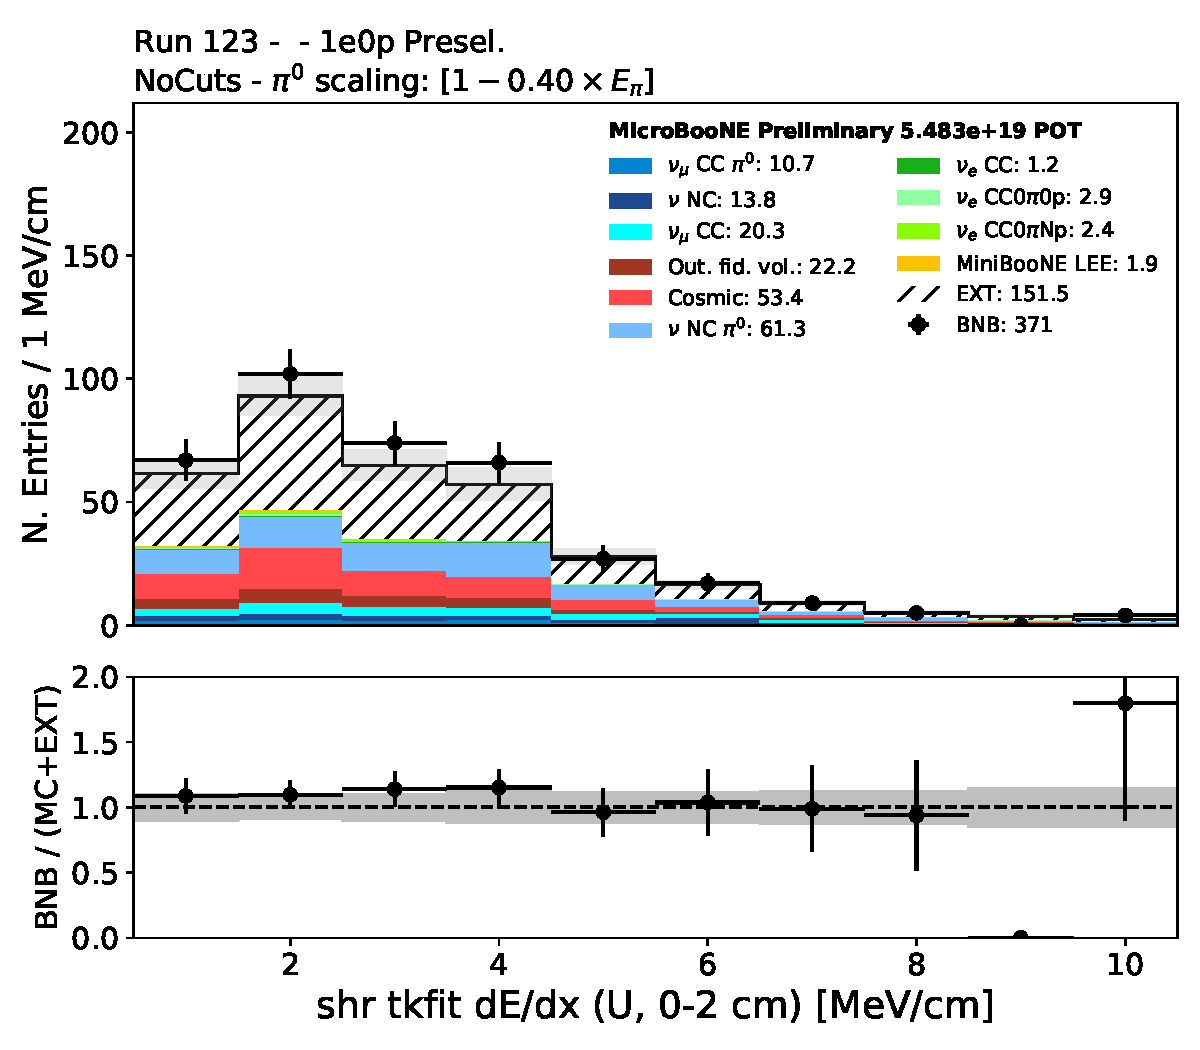
\includegraphics[width=1.00\textwidth]{1e0p/dataMCRun123/shr_tkfit_2cm_dedx_U.pdf}
    \caption{\label{fig:1e0p:dataMCRun1:shr_tkfit_2cm_dedx_U} shr\_tkfit\_2cm\_dedx\_U }
    \end{subfigure}
    \begin{subfigure}[b]{0.3\textwidth}
    \centering
    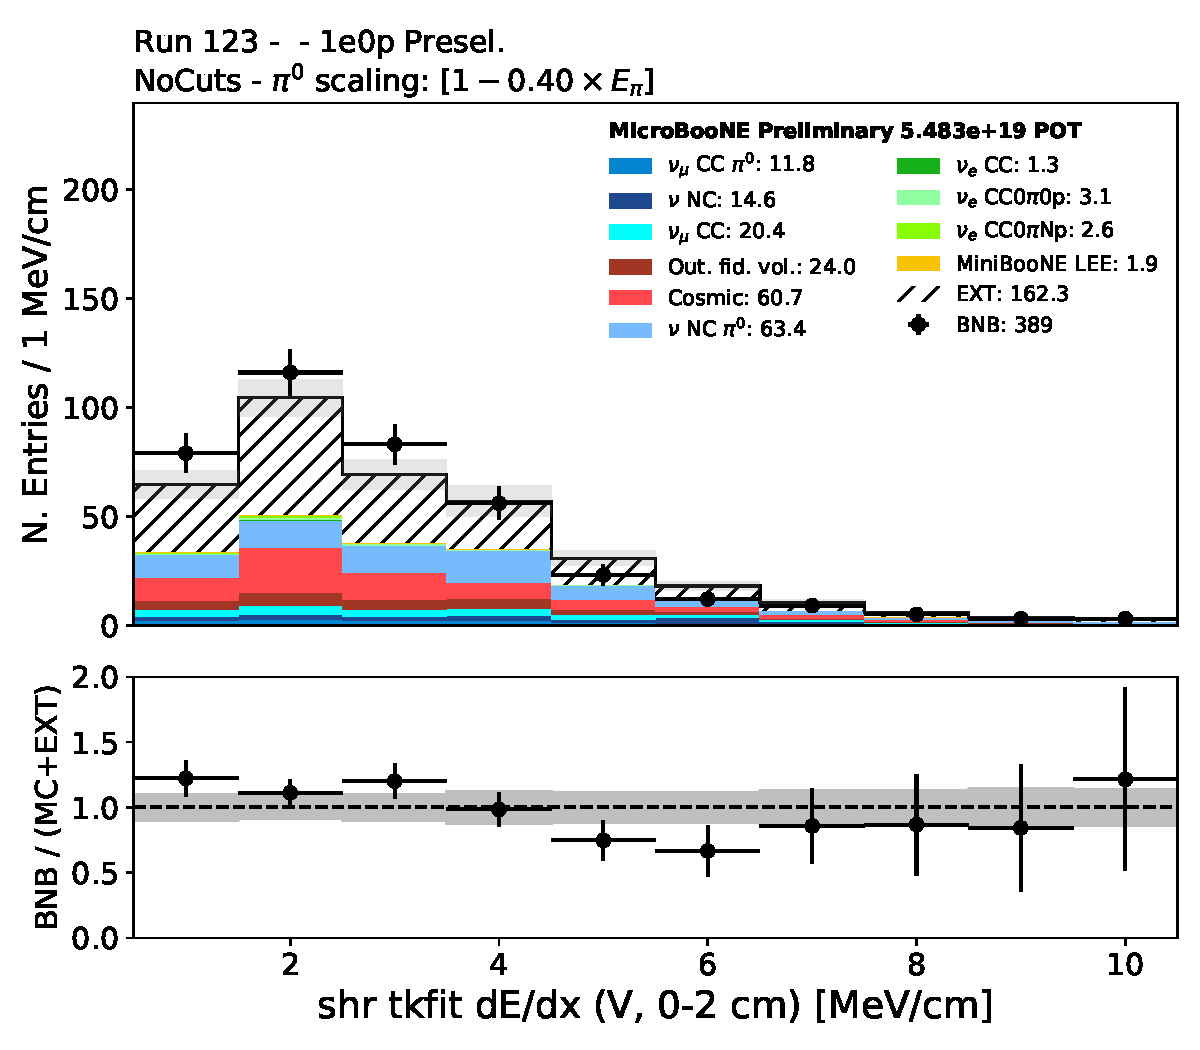
\includegraphics[width=1.00\textwidth]{1e0p/dataMCRun123/shr_tkfit_2cm_dedx_V.pdf}
    \caption{\label{fig:1e0p:dataMCRun1:shr_tkfit_dedx_V} shr\_tkfit\_2cm\_dedx\_V }
    \end{subfigure}
    \begin{subfigure}[b]{0.3\textwidth}
    \centering
    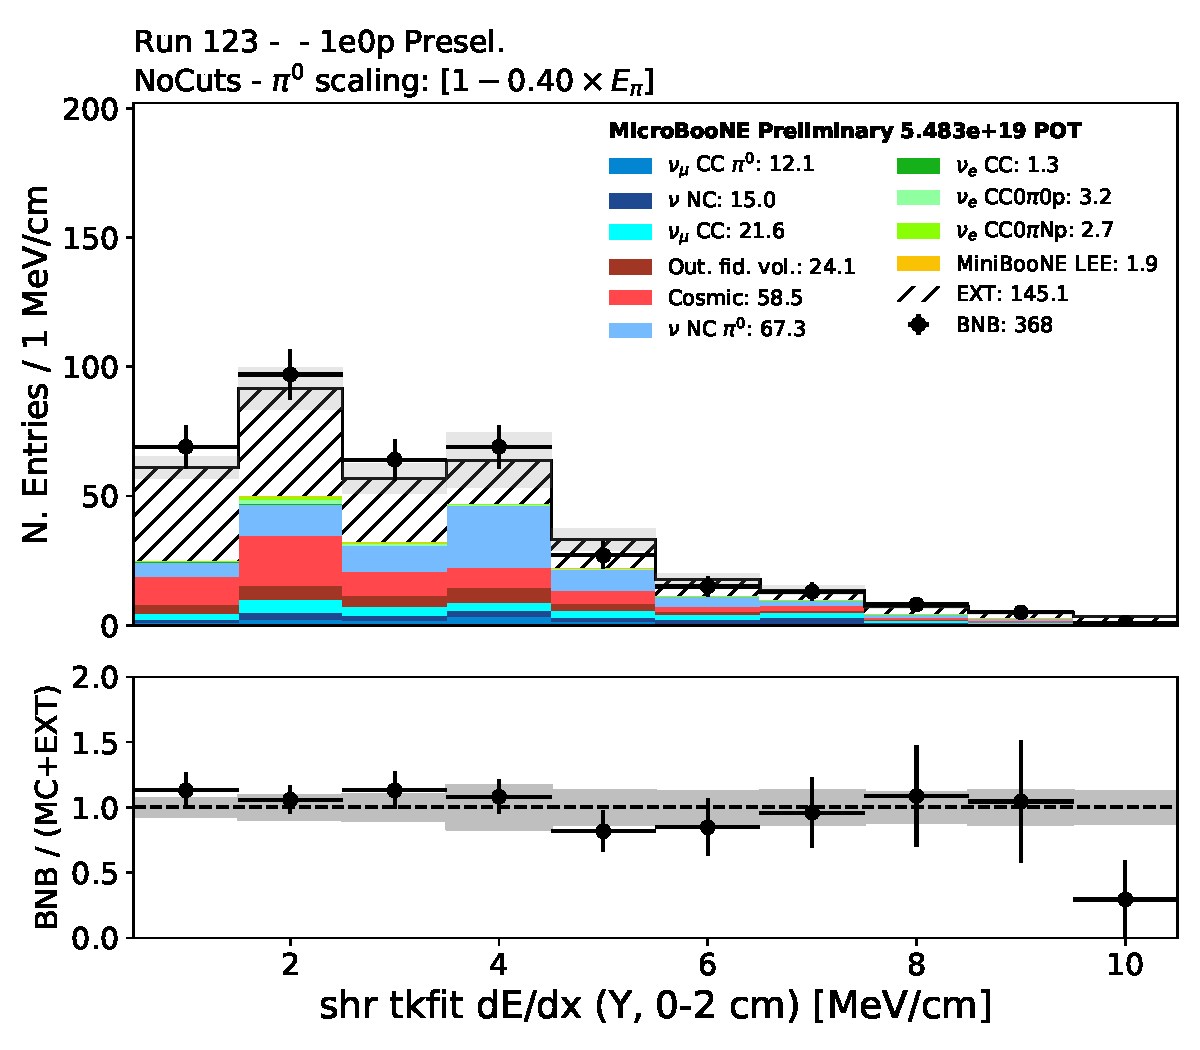
\includegraphics[width=1.00\textwidth]{1e0p/dataMCRun123/shr_tkfit_2cm_dedx_Y.pdf}
    \caption{\label{fig:1e0p:dataMCRun1:shr_tkfit_2cm_dedx_Y} shr\_tkfit\_2cm\_dedx\_Y }
    \end{subfigure}
\caption{\label{fig:1e0p:dataMCRun1:shr_tkfit_dedx_2cm}Data-MC comparison in the open data after the \zpsel preselection.}
\end{center}
\end{figure}

\begin{figure}[H] 
\begin{center}
    \begin{subfigure}[b]{0.3\textwidth}
    \centering
    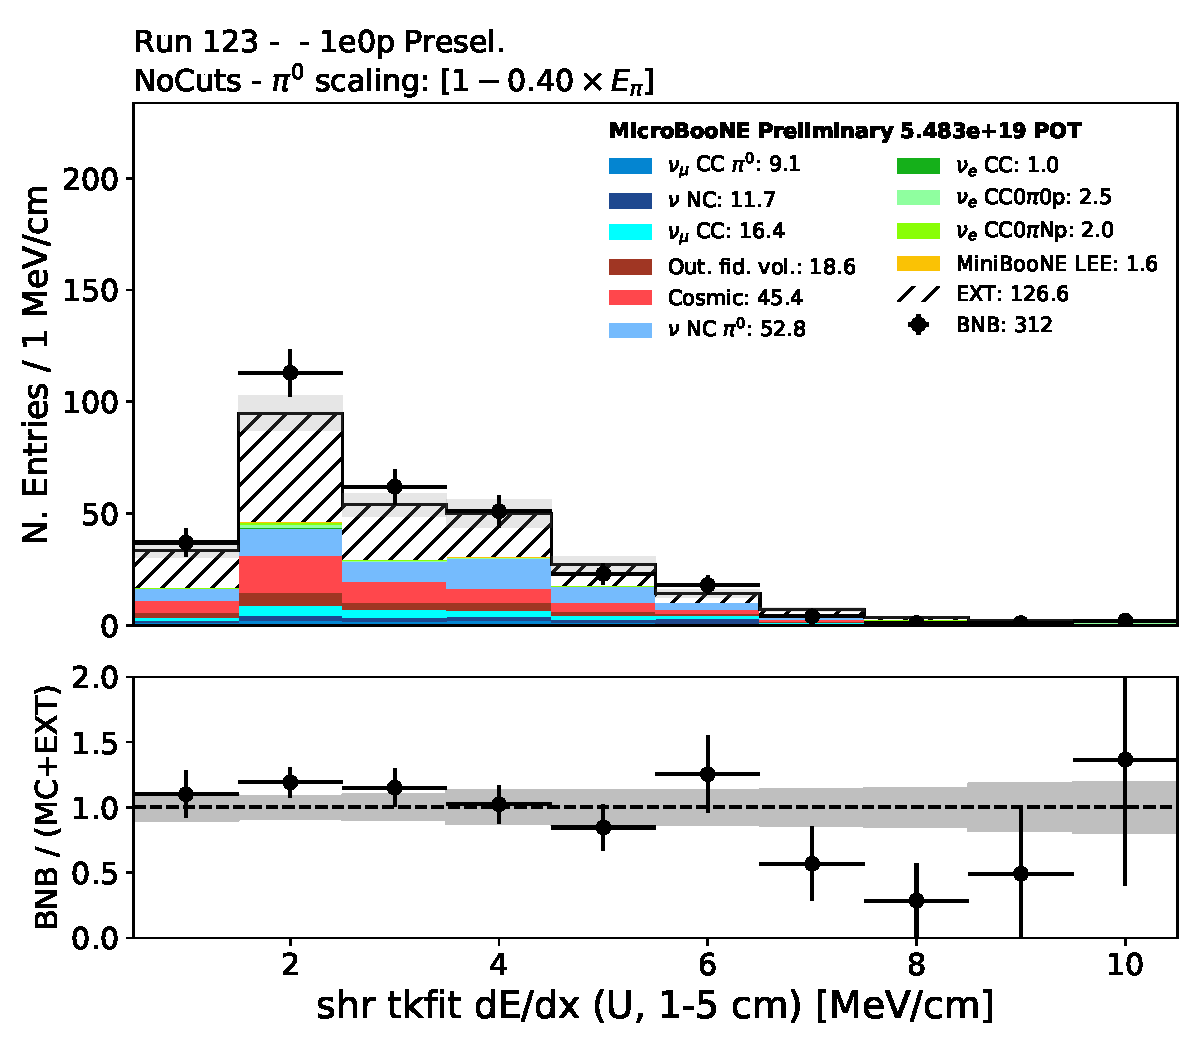
\includegraphics[width=1.00\textwidth]{1e0p/dataMCRun123/shr_tkfit_gap10_dedx_U.pdf}
    \caption{\label{fig:1e0p:dataMCRun1:shr_tkfit_gap10_dedx_U} shr\_tkfit\_gap10\_dedx\_U }
    \end{subfigure}
    \begin{subfigure}[b]{0.3\textwidth}
    \centering
    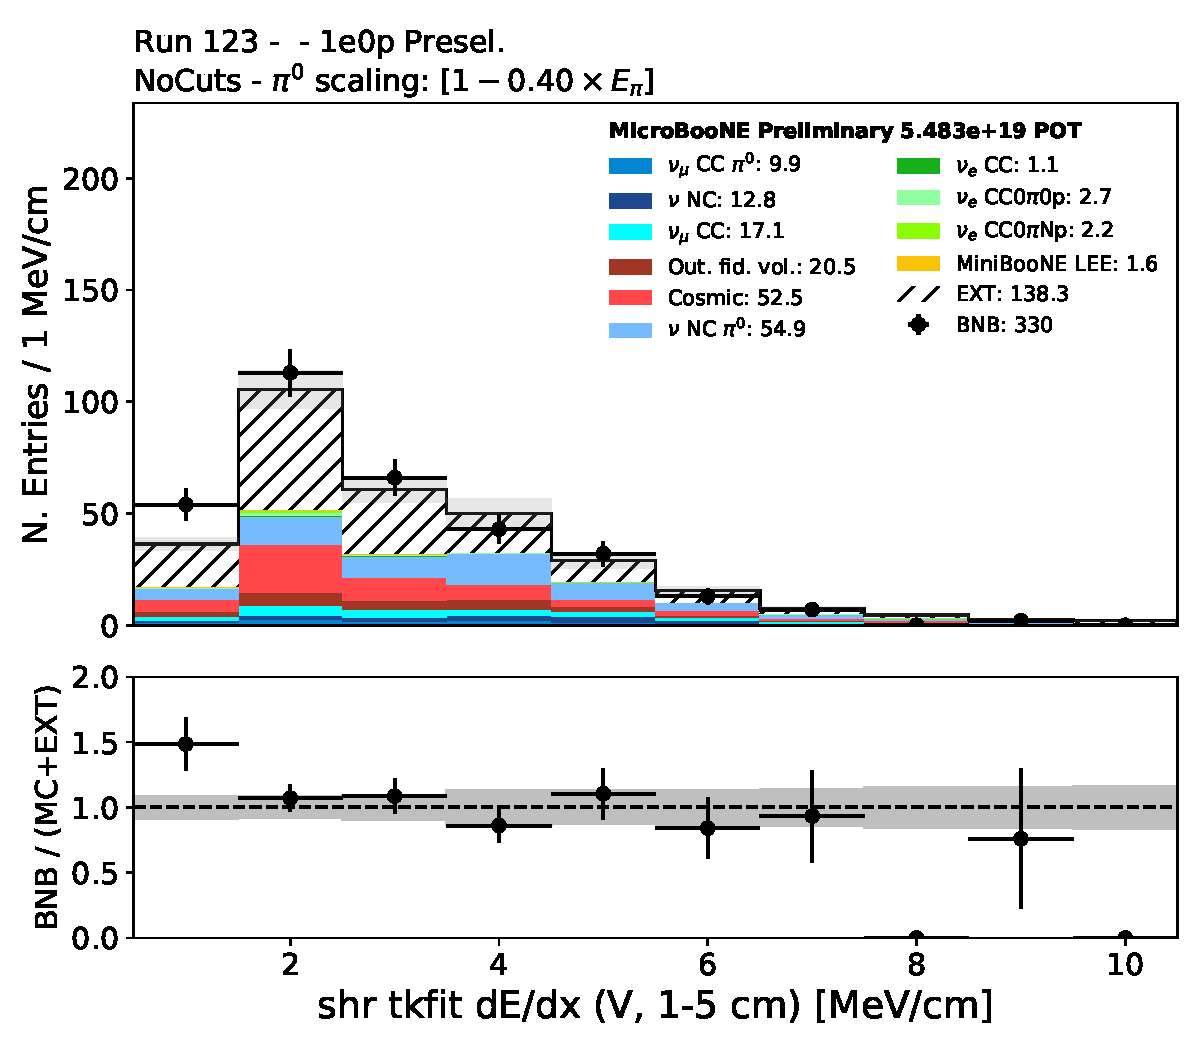
\includegraphics[width=1.00\textwidth]{1e0p/dataMCRun123/shr_tkfit_gap10_dedx_V.pdf}
    \caption{\label{fig:1e0p:dataMCRun1:shr_tkfit_gap10_dedx_V} shr\_tkfit\_gap10\_dedx\_V }
    \end{subfigure}
    \begin{subfigure}[b]{0.3\textwidth}
    \centering
    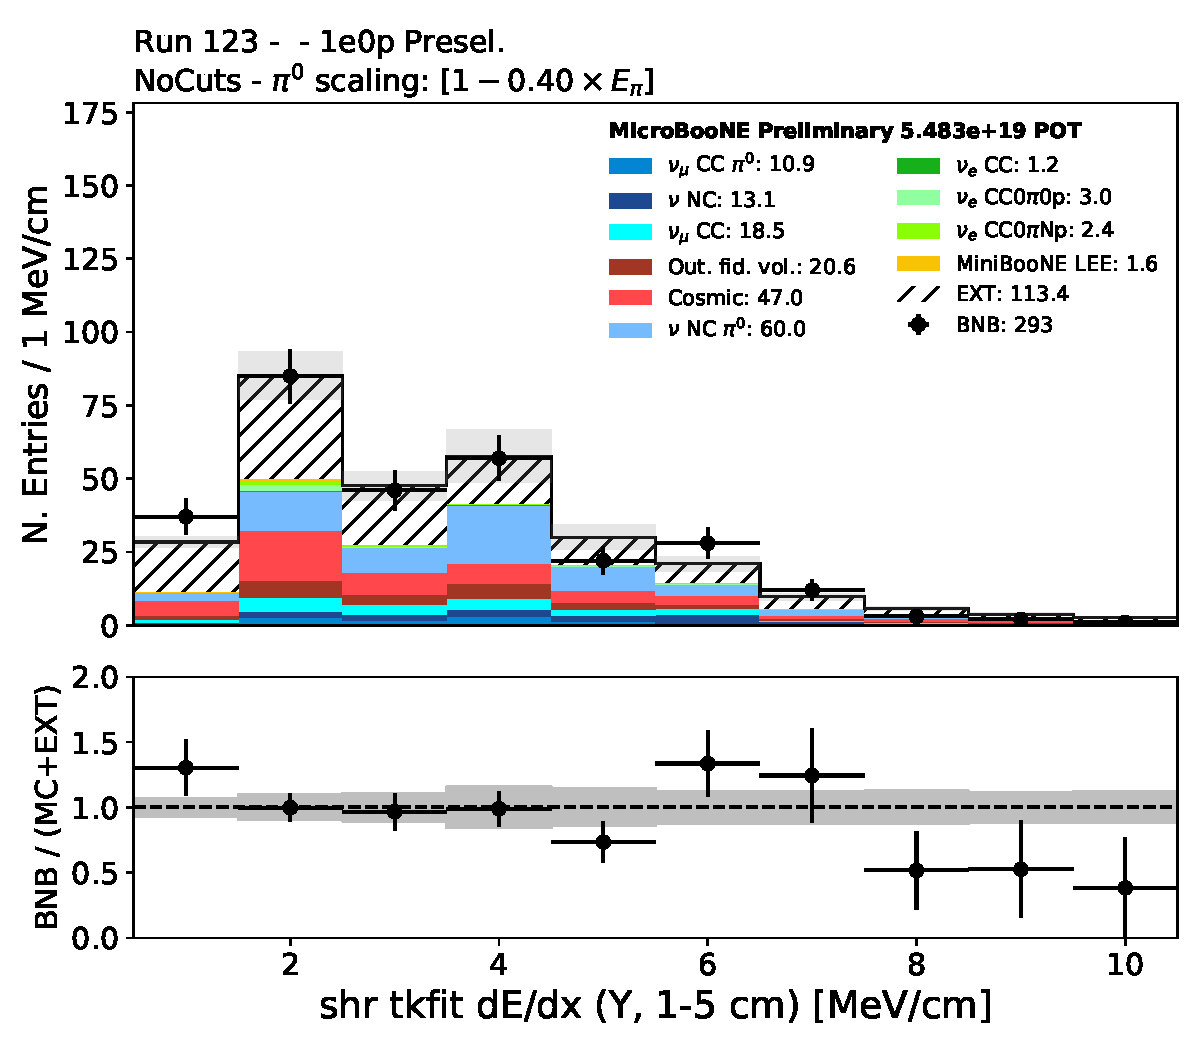
\includegraphics[width=1.00\textwidth]{1e0p/dataMCRun123/shr_tkfit_gap10_dedx_Y.pdf}
    \caption{\label{fig:1e0p:dataMCRun1:shr_tkfit_gap_dedx_Y} shr\_tkfit\_gap10\_dedx\_Y }
    \end{subfigure}
\caption{\label{fig:1e0p:dataMCRun1:shr_tkfit_dedx_2cm}Data-MC comparison in the open data after the \zpsel preselection.}
\end{center}
\end{figure}

\begin{figure}[H] 
\begin{center}
    \begin{subfigure}[b]{0.3\textwidth}
    \centering
    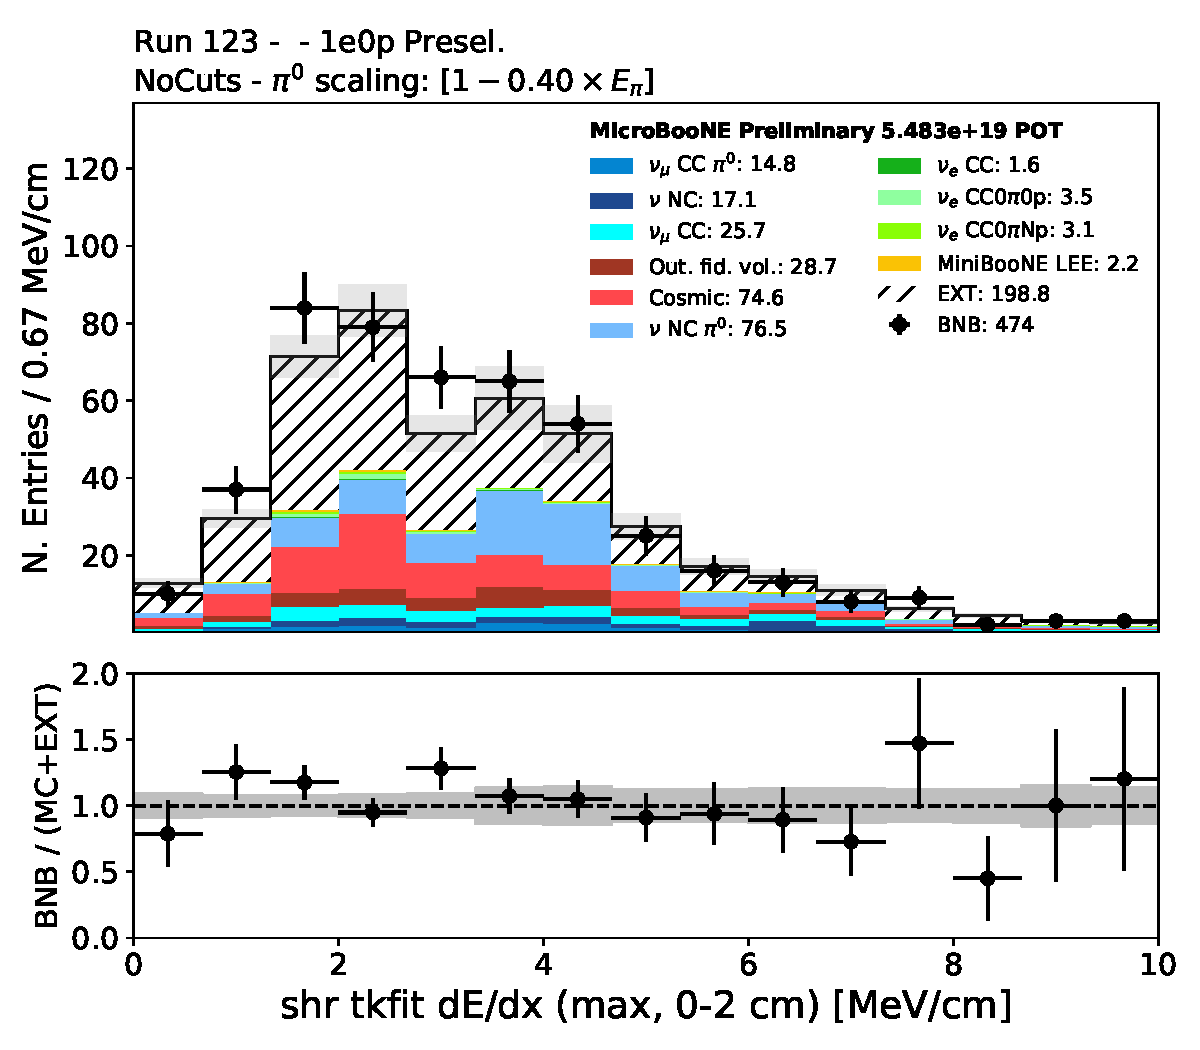
\includegraphics[width=1.00\textwidth]{1e0p/dataMCRun123/shr_tkfit_2cm_dedx_max_opendata_07312020.pdf}
    \caption{\label{fig:1e0p:dataMCRun1:shr_tkfit_gap10_dedx_U} shr\_tkfit\_2cm\_dedx\_max }
    \end{subfigure}
    \begin{subfigure}[b]{0.3\textwidth}
    \centering
    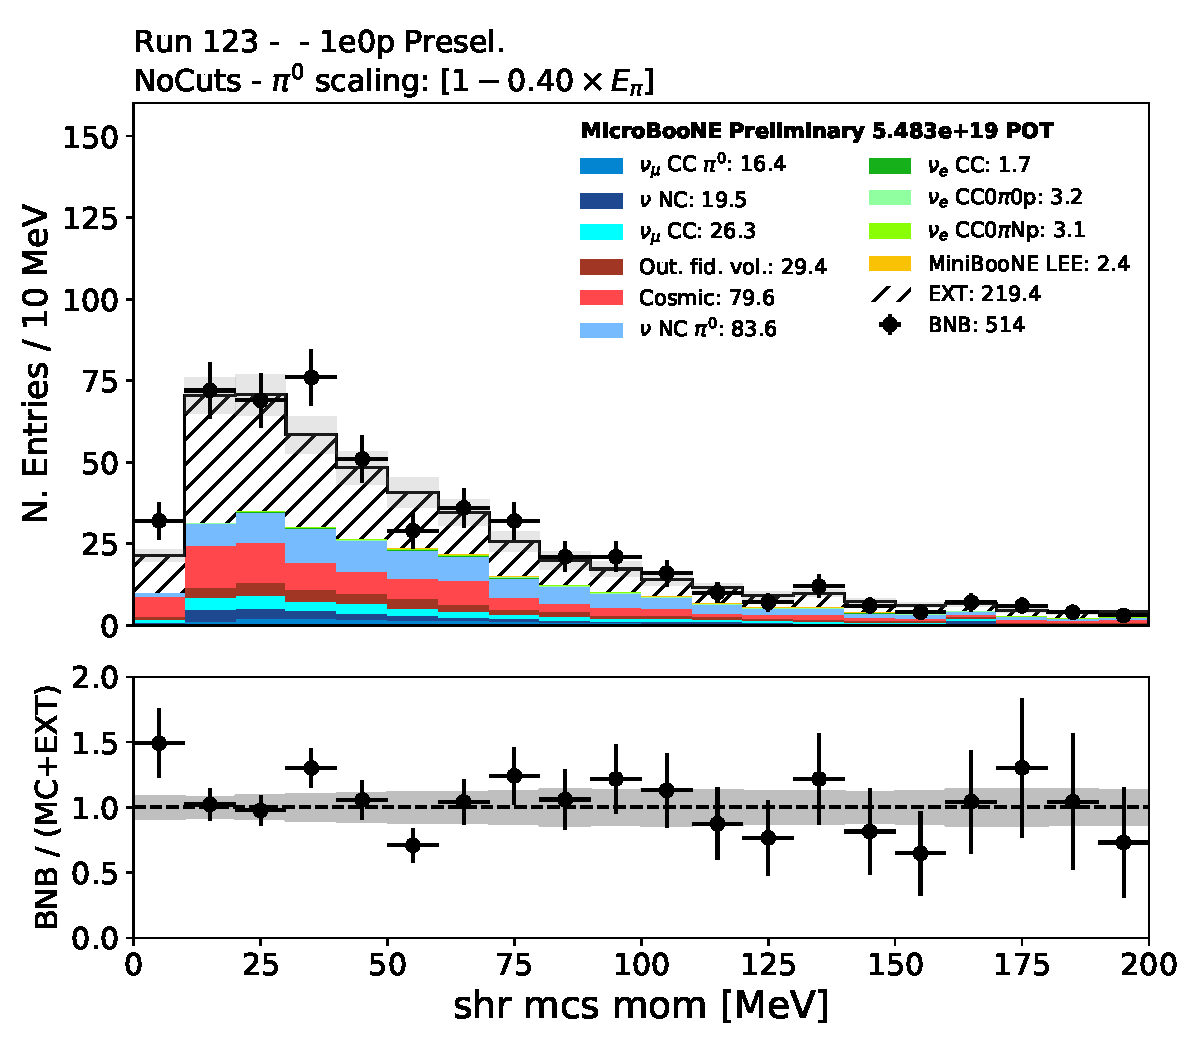
\includegraphics[width=1.00\textwidth]{1e0p/dataMCRun123/shrMCSMom.pdf}
    \caption{\label{fig:1e0p:dataMCRun1:shr_tkfit_gap10_dedx_V} shrMCSMom }
    \end{subfigure}
    \begin{subfigure}[b]{0.3\textwidth}
    \centering
    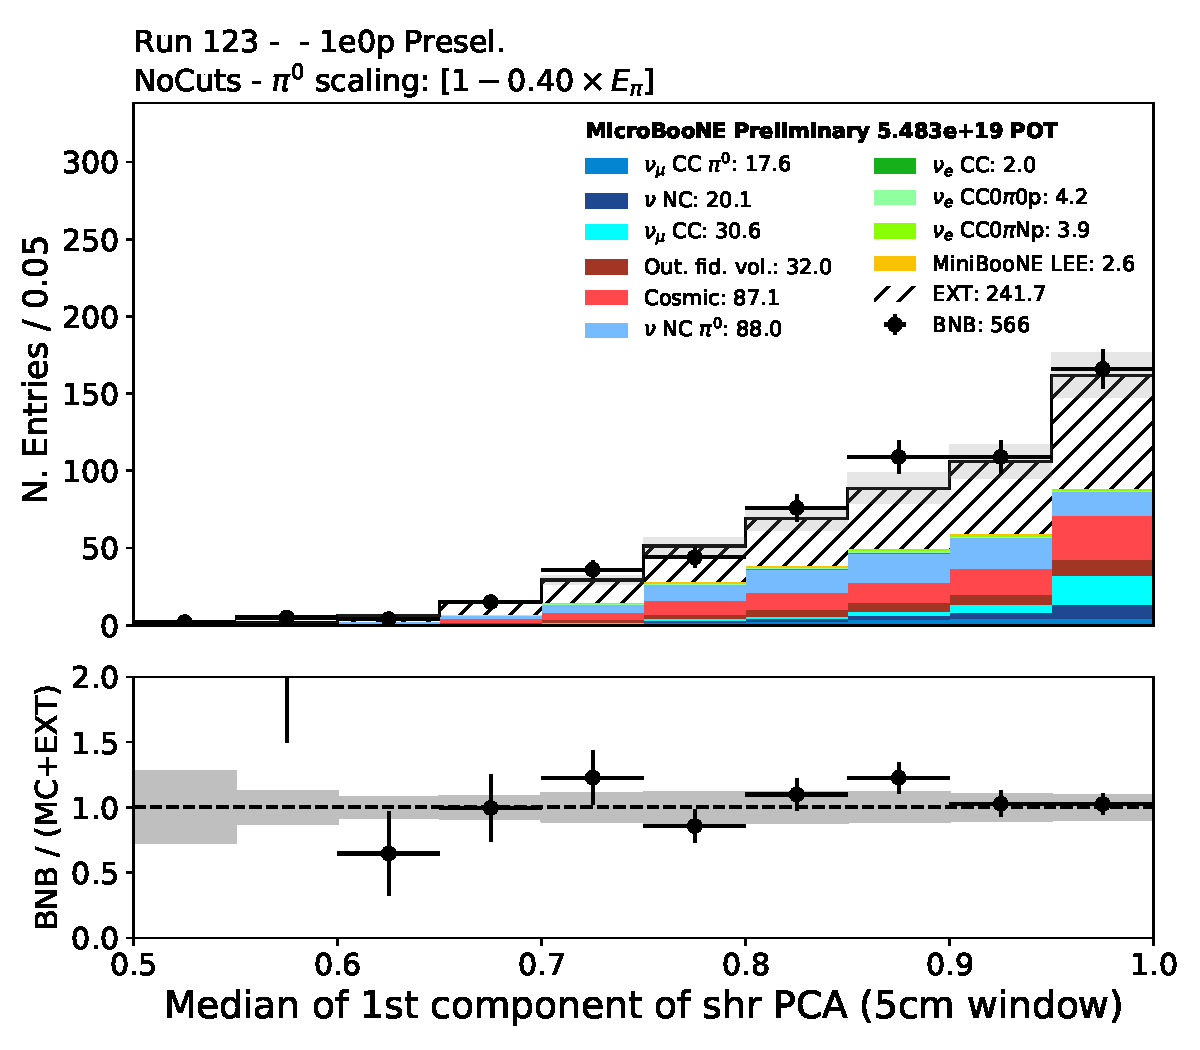
\includegraphics[width=1.00\textwidth]{1e0p/dataMCRun123/shrPCA1CMed_5cm.pdf}
    \caption{\label{fig:1e0p:dataMCRun1:shr_tkfit_gap_dedx_Y} shrPCA1CMed\_5cm}
    \end{subfigure}
\caption{\label{fig:1e0p:dataMCRun1:shr_tkfit_dedx_2cm}Data-MC comparison in the open data after the \zpsel preselection.}
\end{center}
\end{figure}

\begin{figure}[H] 
\begin{center}
    \begin{subfigure}[b]{0.3\textwidth}
    \centering
    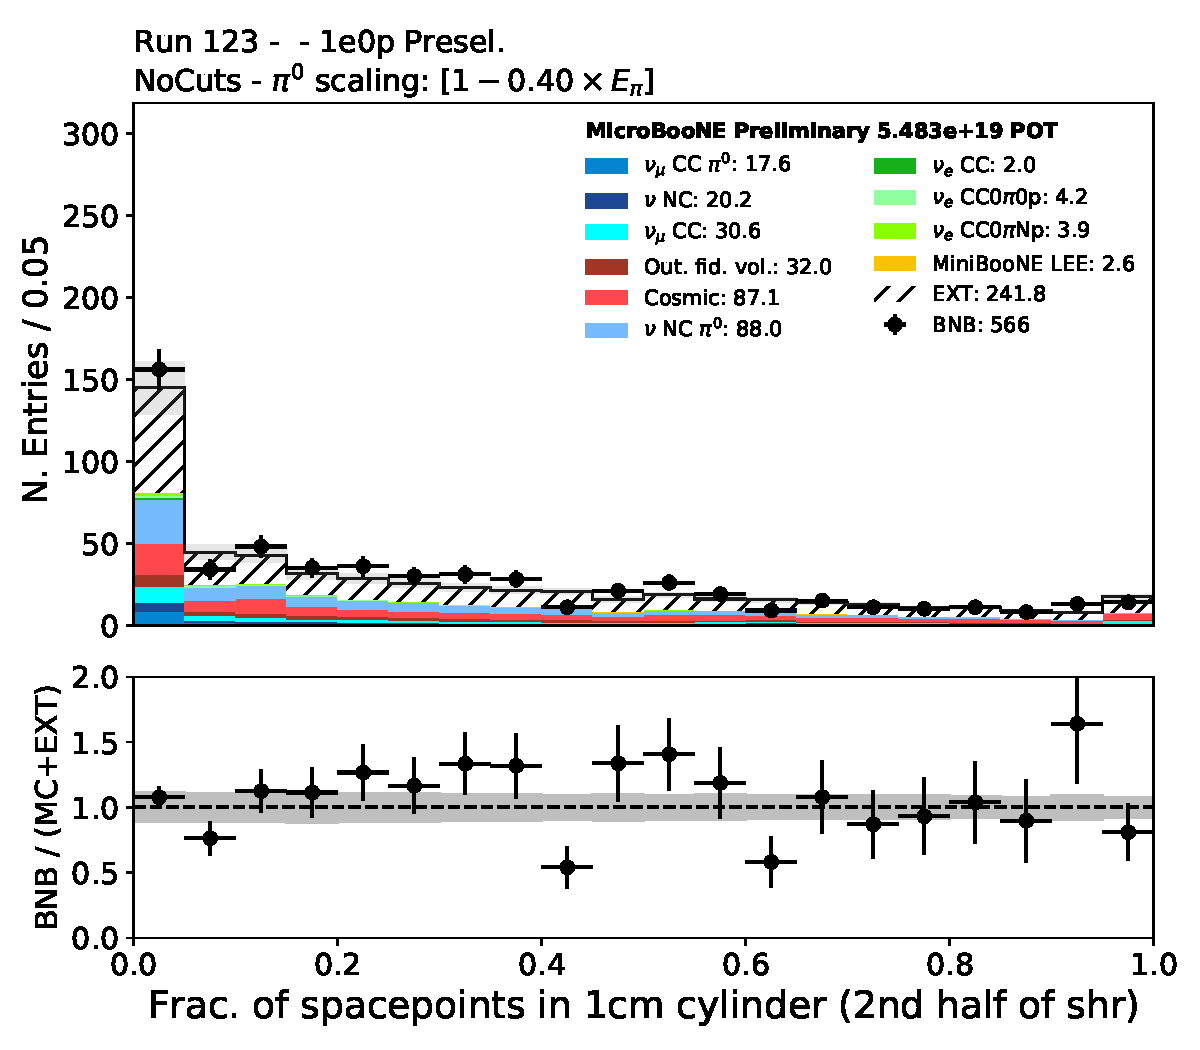
\includegraphics[width=1.00\textwidth]{1e0p/dataMCRun123/CylFrac2h_1cm.pdf}
    \caption{\label{fig:1e0p:dataMCRun1:shr_tkfit_gap10_dedx_U} CylFrac2h\_1cm }
    \end{subfigure}
    \begin{subfigure}[b]{0.3\textwidth}
    \centering
    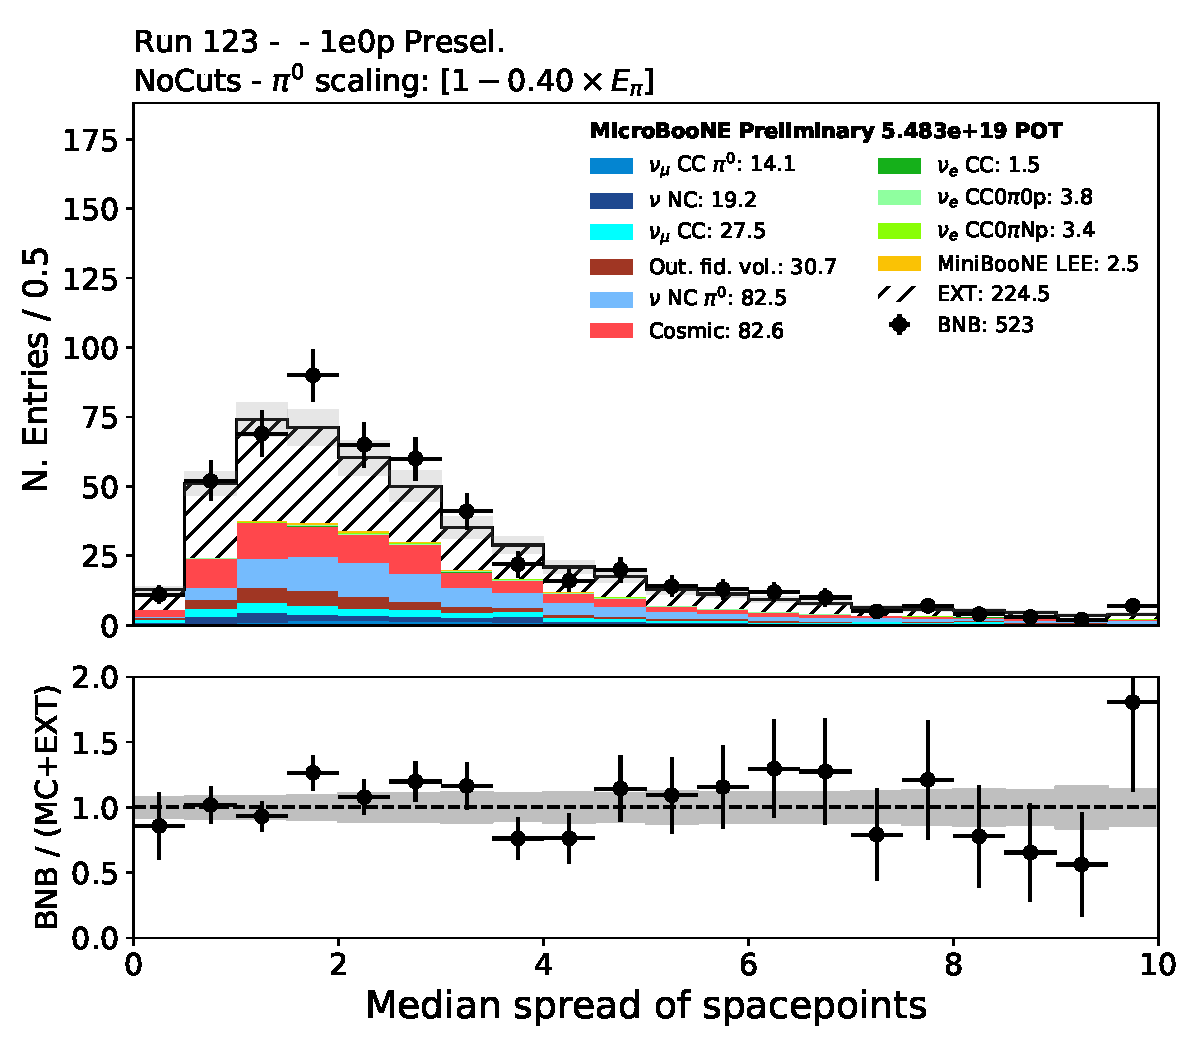
\includegraphics[width=1.00\textwidth]{1e0p/dataMCRun123/DeltaRMS2h.pdf}
    \caption{\label{fig:1e0p:dataMCRun1:shr_tkfit_gap10_dedx_U} CylFrac2h\_1cm }
    \end{subfigure}
\caption{\label{fig:1e0p:dataMCRun1:shr_tkfit_dedx_2cm}Data-MC comparison in the open data after the \zpsel preselection.}
\end{center}
\end{figure}

\begin{figure}[H] 
\begin{center}
    \begin{subfigure}[b]{0.3\textwidth}
    \centering
    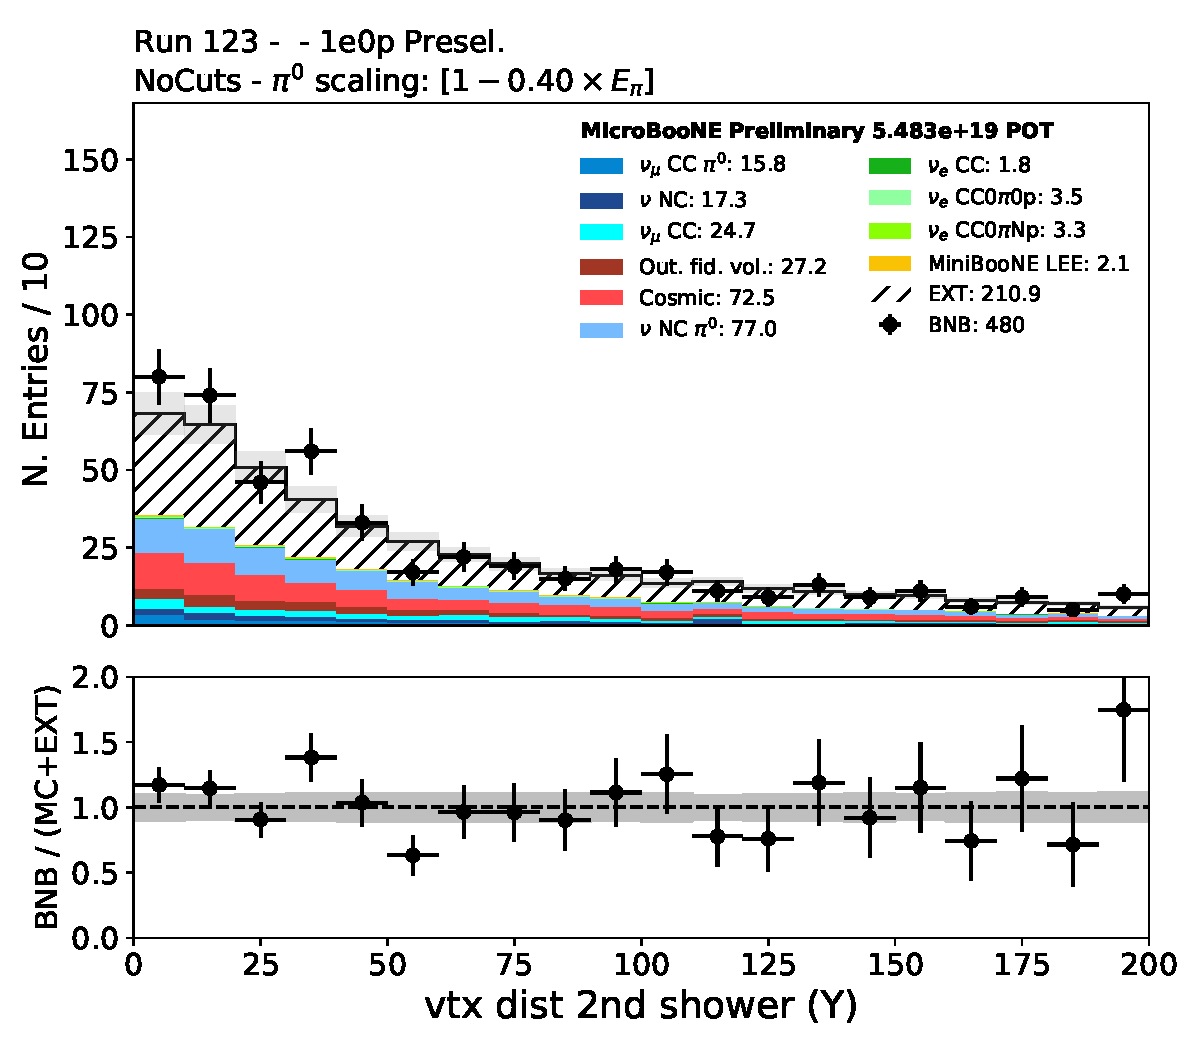
\includegraphics[width=1.00\textwidth]{1e0p/dataMCRun123/secondshower_Y_vtxdist.pdf}
    \caption{\label{fig:1e0p:dataMCRun1:secondshower_Y_vtxdist} secondshower\_Y\_vtxdist }
    \end{subfigure}
    \begin{subfigure}[b]{0.3\textwidth}
    \centering
    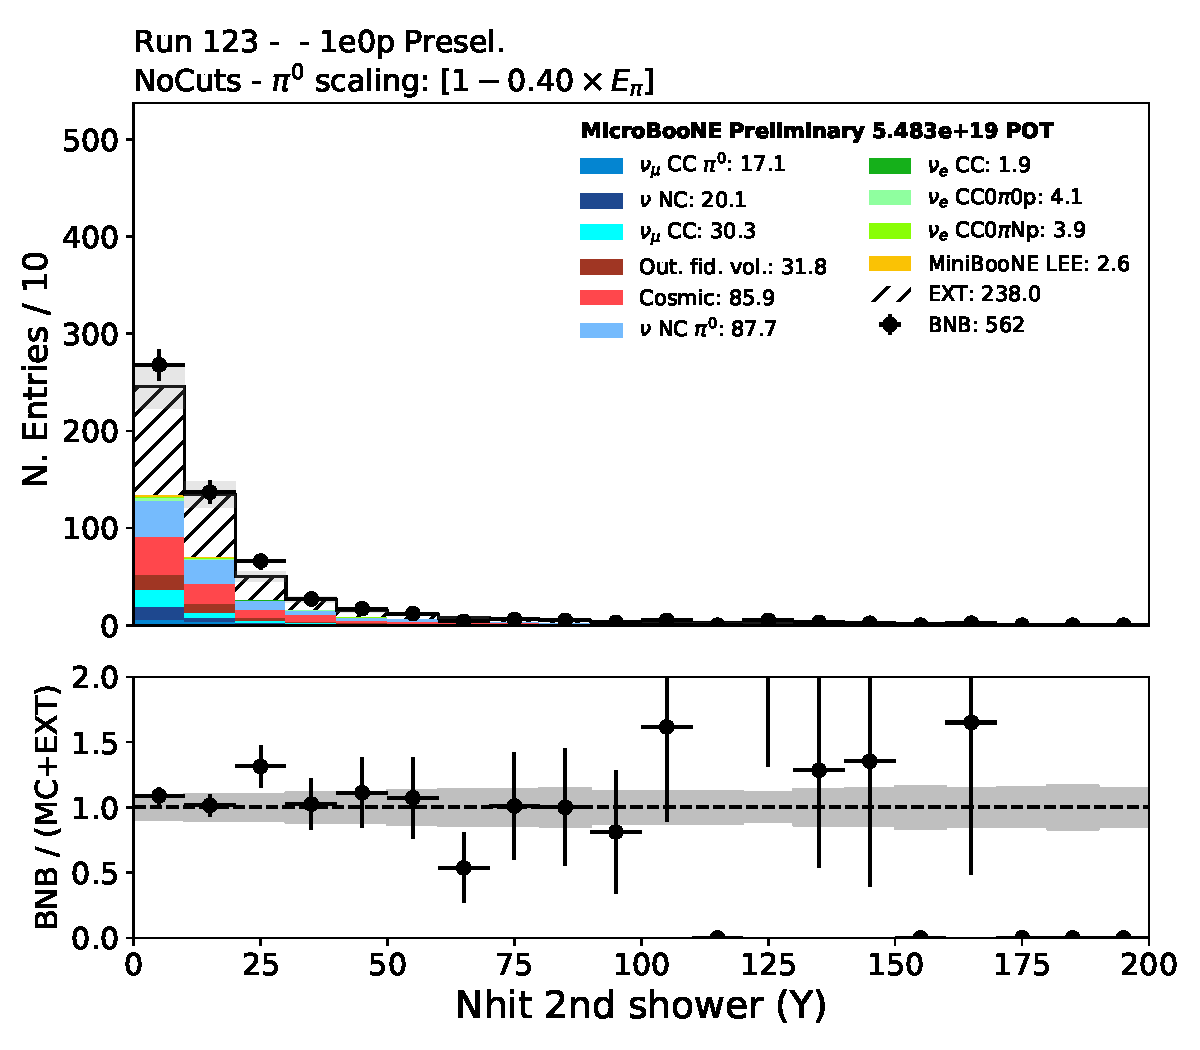
\includegraphics[width=1.00\textwidth]{1e0p/dataMCRun123/secondshower_Y_nhit.pdf}
    \caption{\label{fig:1e0p:dataMCRun1:secondshower_Y_nhit} secondshower\_Y\_nhit }
    \end{subfigure}
\caption{\label{fig:1e0p:dataMCRun1:pi01}Data-MC comparison in the open data after the \zpsel preselection.}
\end{center}
\end{figure}

\begin{figure}[H] 
\begin{center}
    \begin{subfigure}[b]{0.3\textwidth}
    \centering
    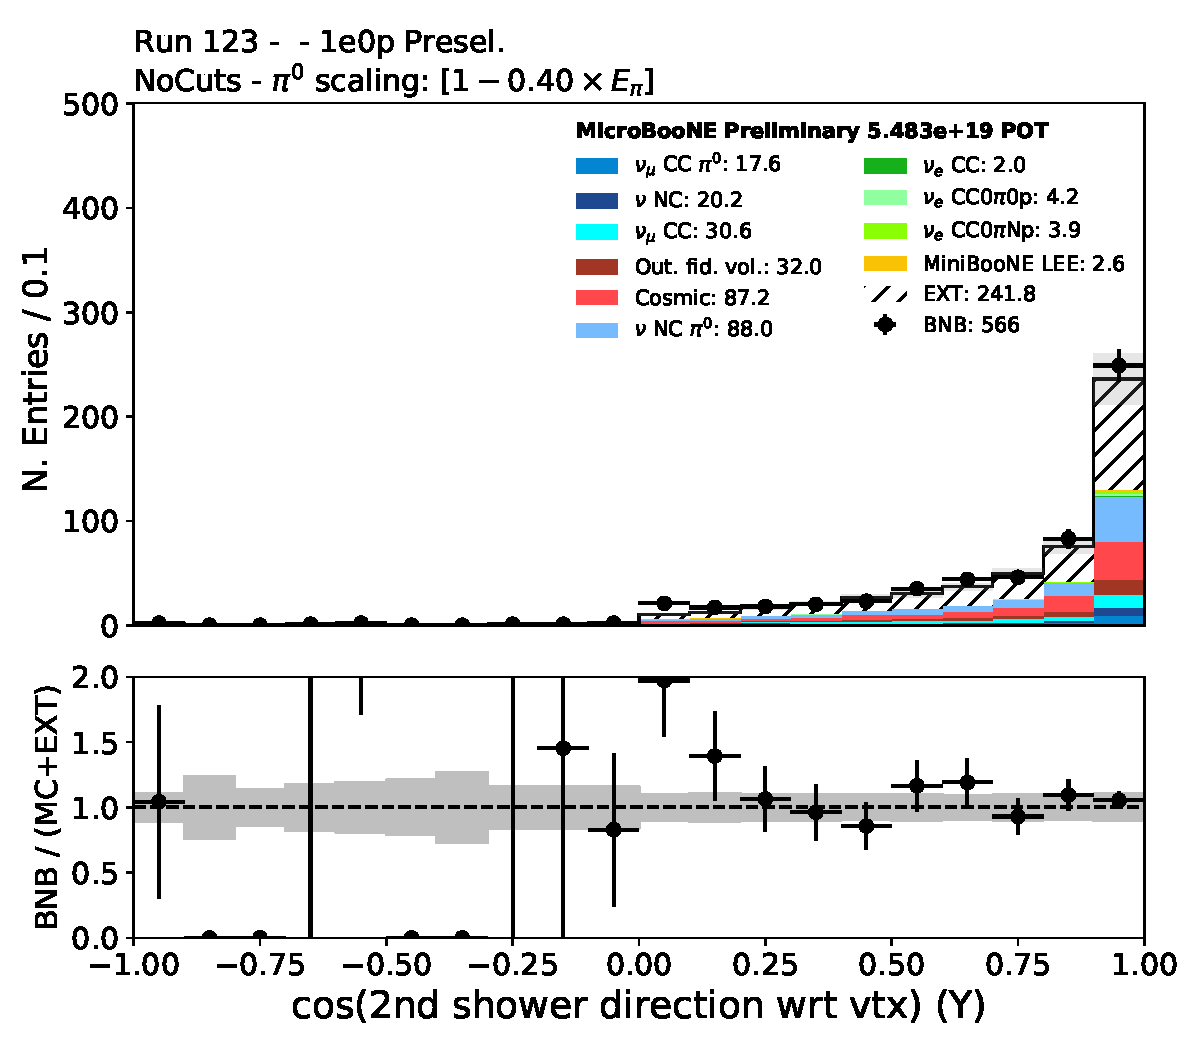
\includegraphics[width=1.00\textwidth]{1e0p/dataMCRun123/secondshower_Y_dot.pdf}
    \caption{\label{fig:1e0p:dataMCRun1:secondshower_Y_dot} secondshower\_Y\_dot }
    \end{subfigure}
    \begin{subfigure}[b]{0.3\textwidth}
    \centering
    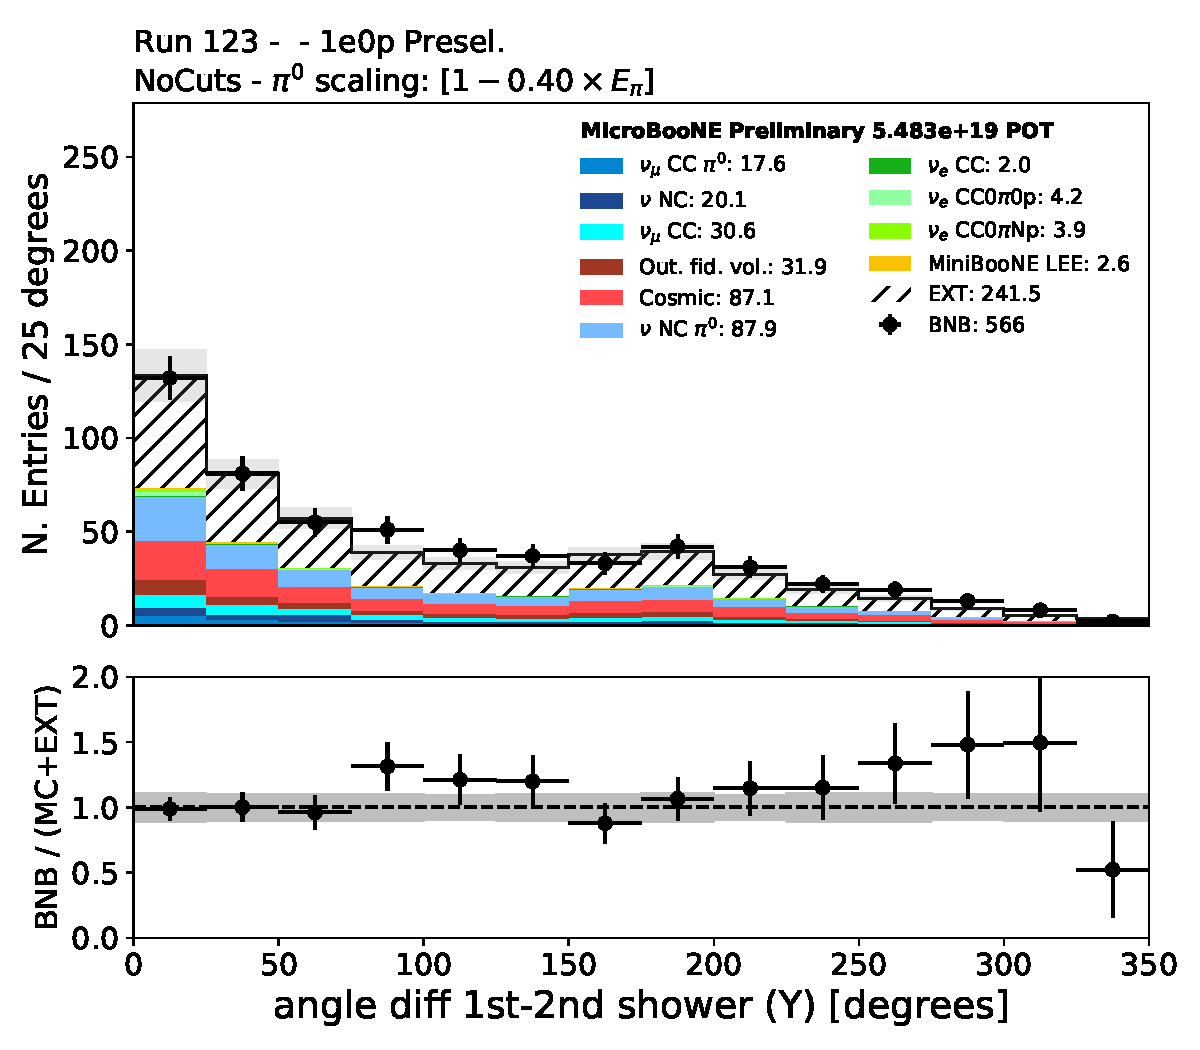
\includegraphics[width=1.00\textwidth]{1e0p/dataMCRun123/anglediff_Y.pdf}
    \caption{\label{fig:1e0p:dataMCRun1:anglediff_Y} anglediff\_Y }
    \end{subfigure}
\caption{\label{fig:1e0p:dataMCRun1:pi02}Data-MC comparison in the open data after the \zpsel preselection.}
\end{center}
\end{figure}

\begin{figure}[H] 
\begin{center}
    \begin{subfigure}[b]{0.3\textwidth}
    \centering
    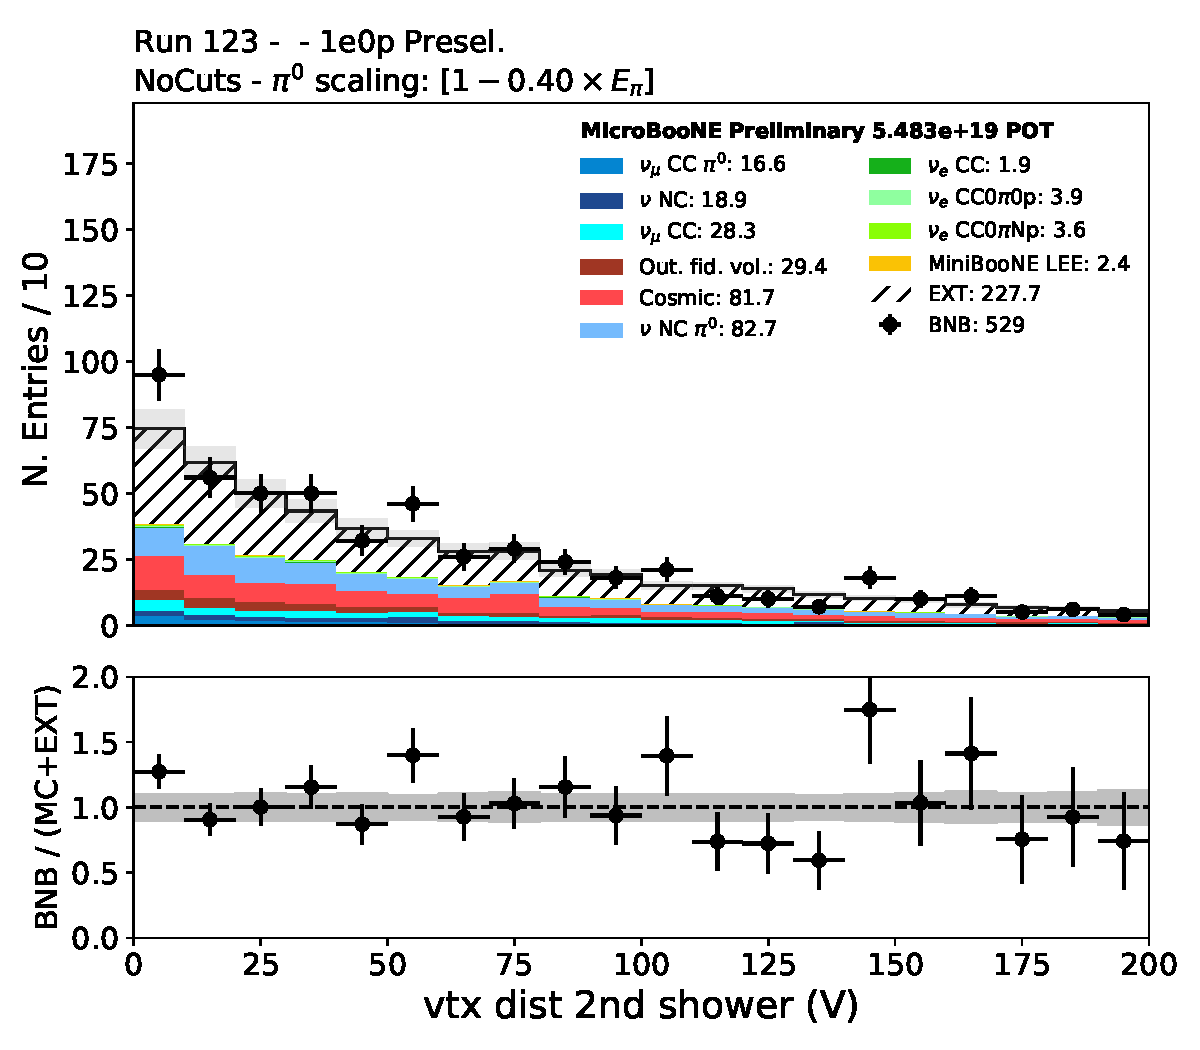
\includegraphics[width=1.00\textwidth]{1e0p/dataMCRun123/secondshower_V_vtxdist.pdf}
    \caption{\label{fig:1e0p:dataMCRun1:secondshower_V_vtxdist} secondshower\_V\_vtxdist }
    \end{subfigure}
    \begin{subfigure}[b]{0.3\textwidth}
    \centering
    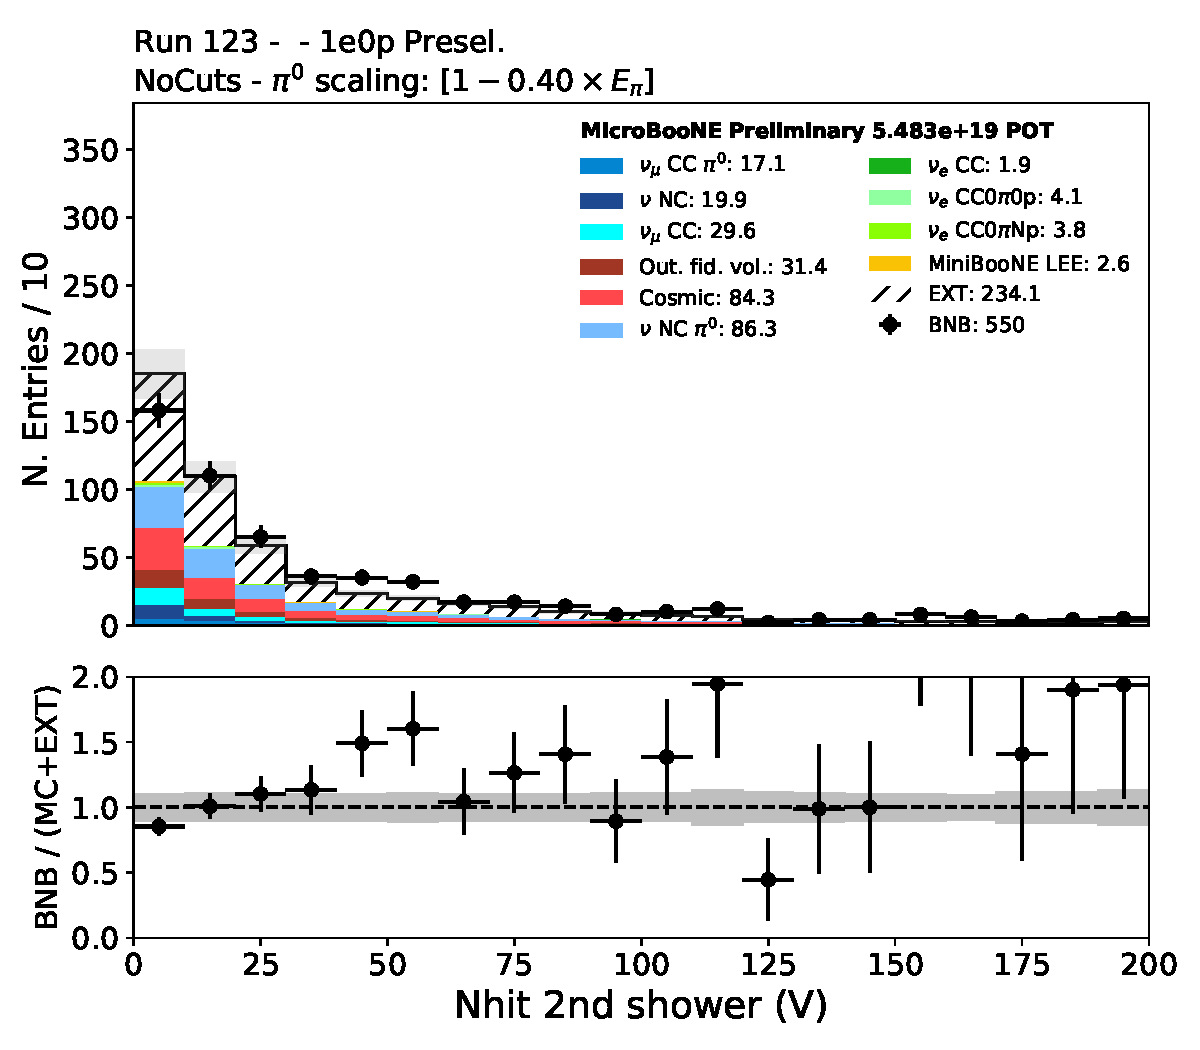
\includegraphics[width=1.00\textwidth]{1e0p/dataMCRun123/secondshower_V_nhit.pdf}
    \caption{\label{fig:1e0p:dataMCRun1:secondshower_V_nhit} secondshower\_V\_nhit }
    \end{subfigure}
\caption{\label{fig:1e0p:dataMCRun1:pi01}Data-MC comparison in the open data after the \zpsel preselection.}
\end{center}
\end{figure}

\begin{figure}[H] 
\begin{center}
    \begin{subfigure}[b]{0.3\textwidth}
    \centering
    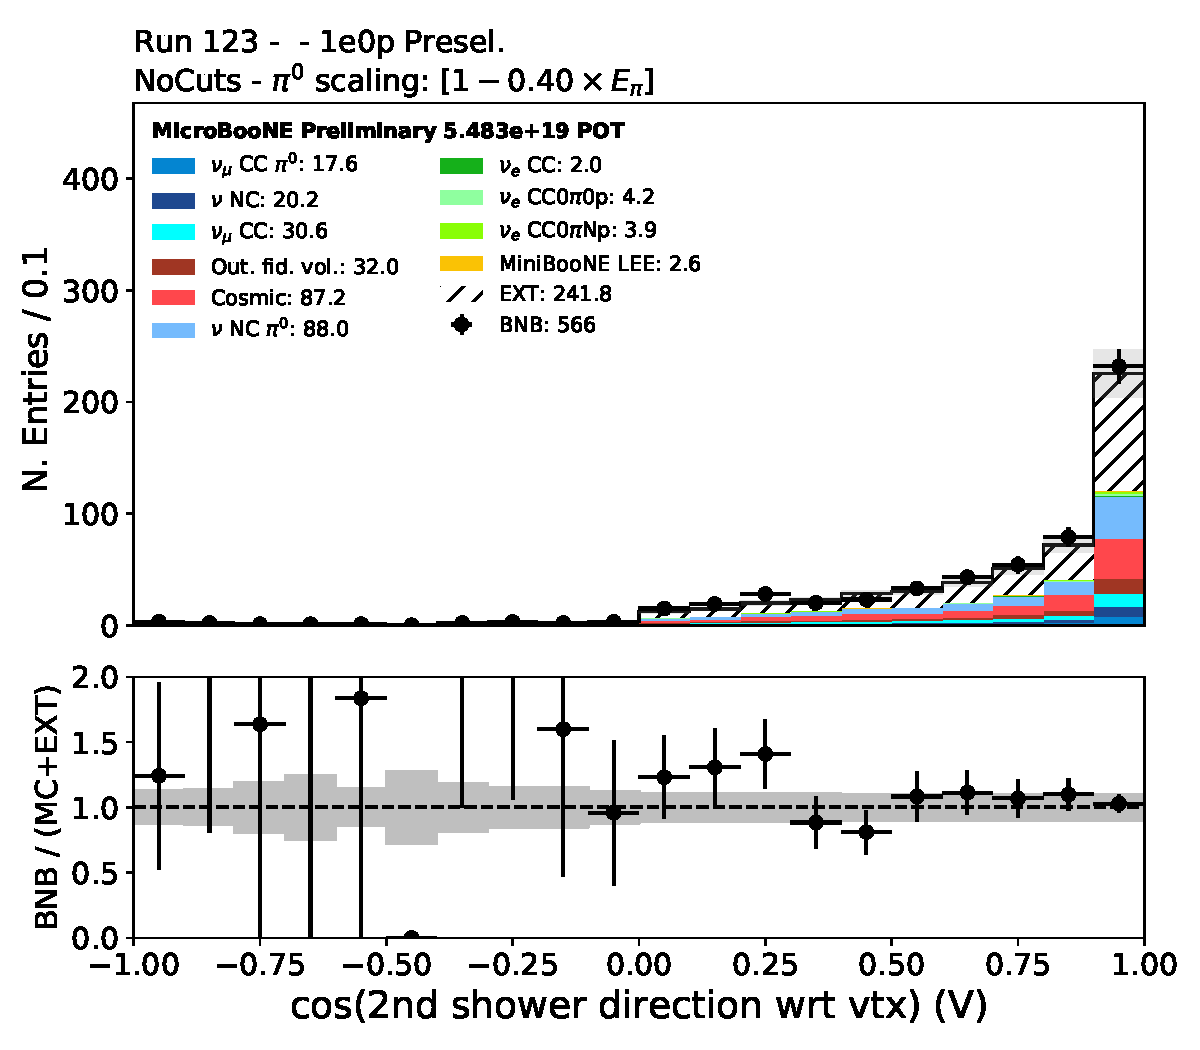
\includegraphics[width=1.00\textwidth]{1e0p/dataMCRun123/secondshower_V_dot.pdf}
    \caption{\label{fig:1e0p:dataMCRun1:secondshower_V_dot} secondshower\_V\_dot }
    \end{subfigure}
    \begin{subfigure}[b]{0.3\textwidth}
    \centering
    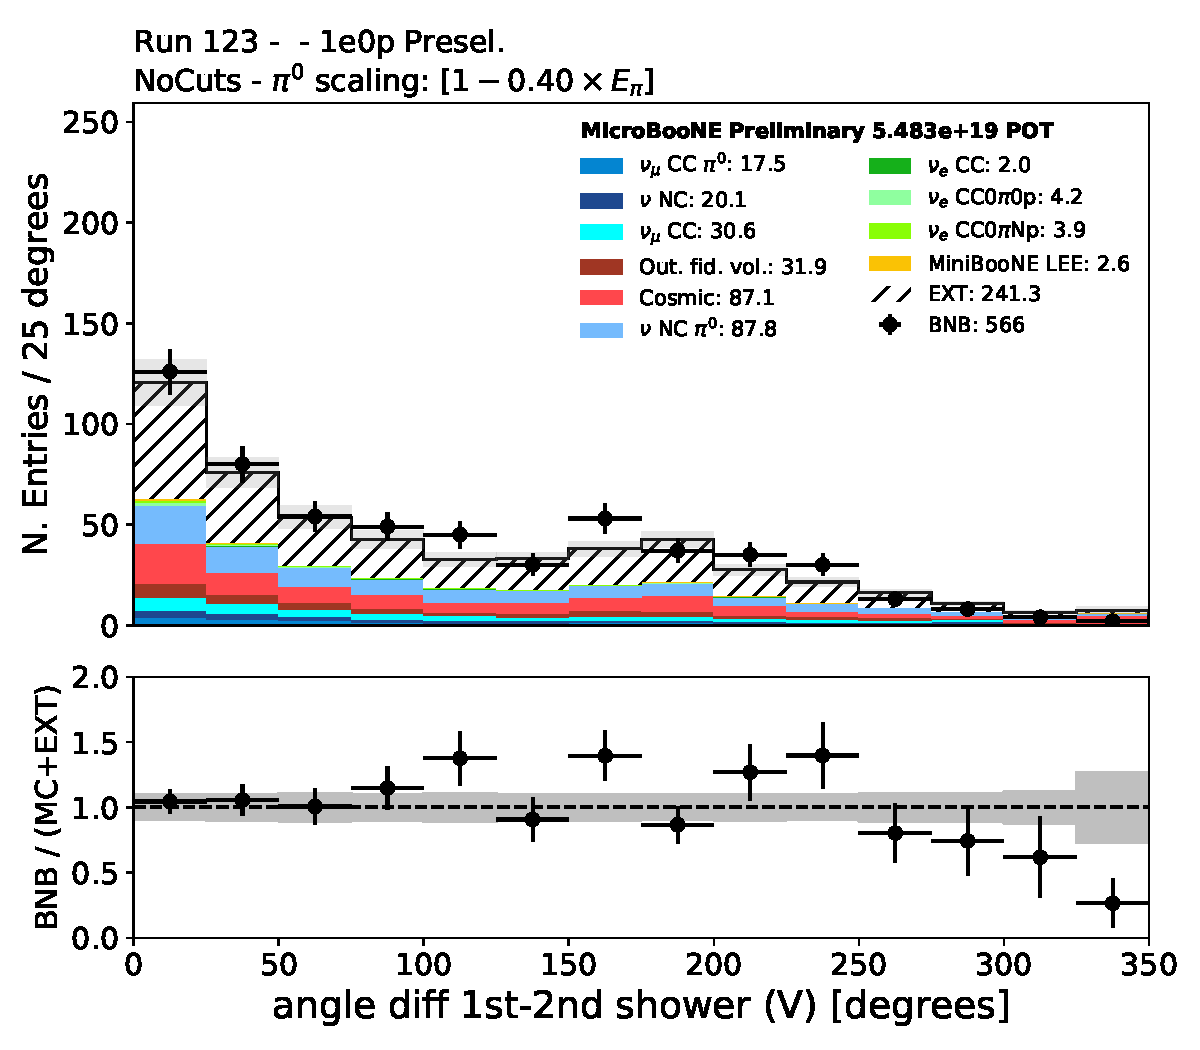
\includegraphics[width=1.00\textwidth]{1e0p/dataMCRun123/anglediff_V.pdf}
    \caption{\label{fig:1e0p:dataMCRun1:anglediff_V} anglediff\_V }
    \end{subfigure}
\caption{\label{fig:1e0p:dataMCRun1:pi02}Data-MC comparison in the open data after the \zpsel preselection.}
\end{center}
\end{figure}

\begin{figure}[H] 
\begin{center}
    \begin{subfigure}[b]{0.3\textwidth}
    \centering
    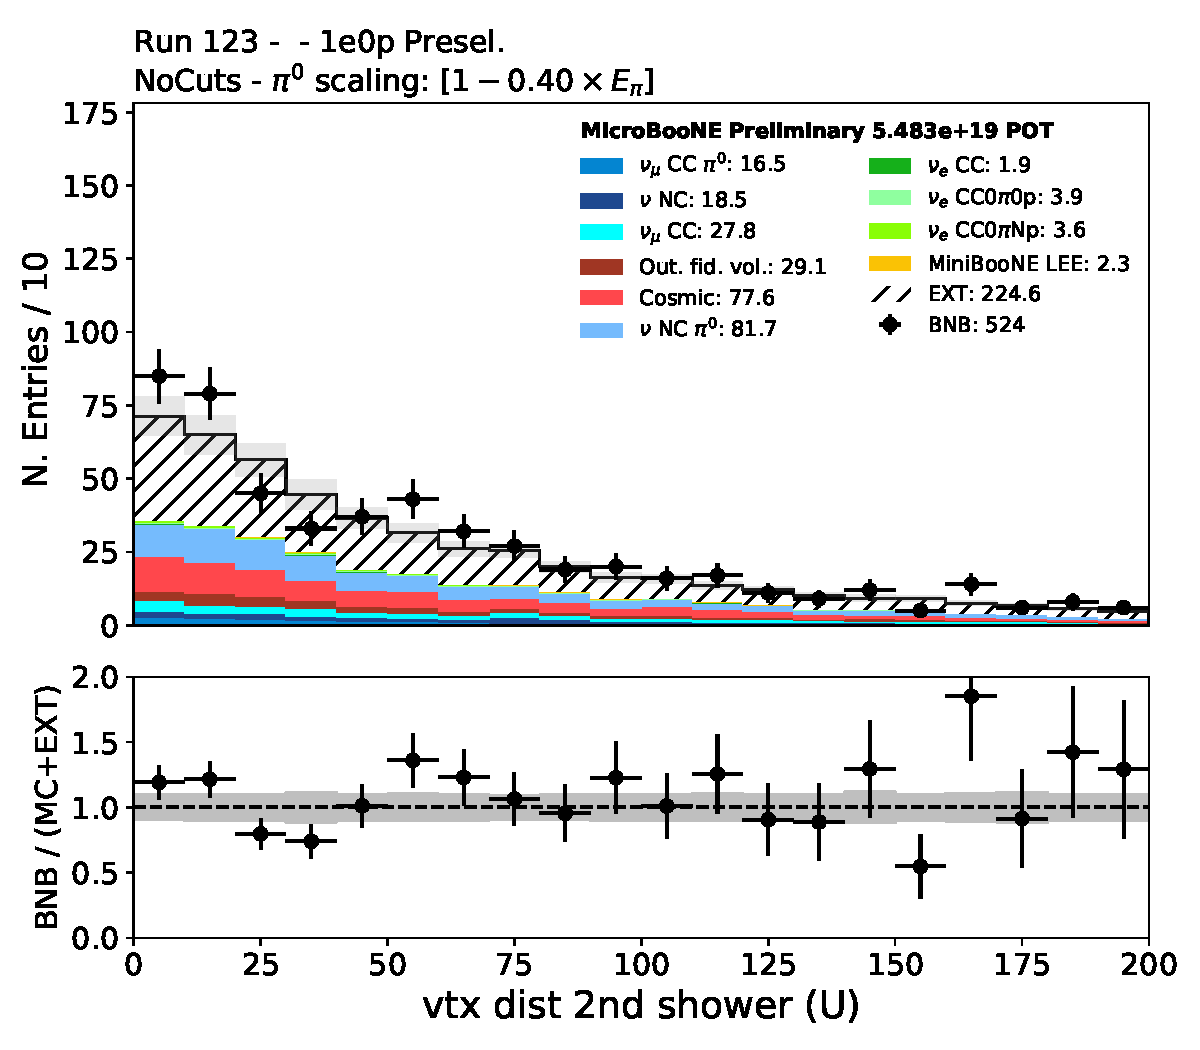
\includegraphics[width=1.00\textwidth]{1e0p/dataMCRun123/secondshower_U_vtxdist.pdf}
    \caption{\label{fig:1e0p:dataMCRun1:secondshower_U_vtxdist} secondshower\_U\_vtxdist }
    \end{subfigure}
    \begin{subfigure}[b]{0.3\textwidth}
    \centering
    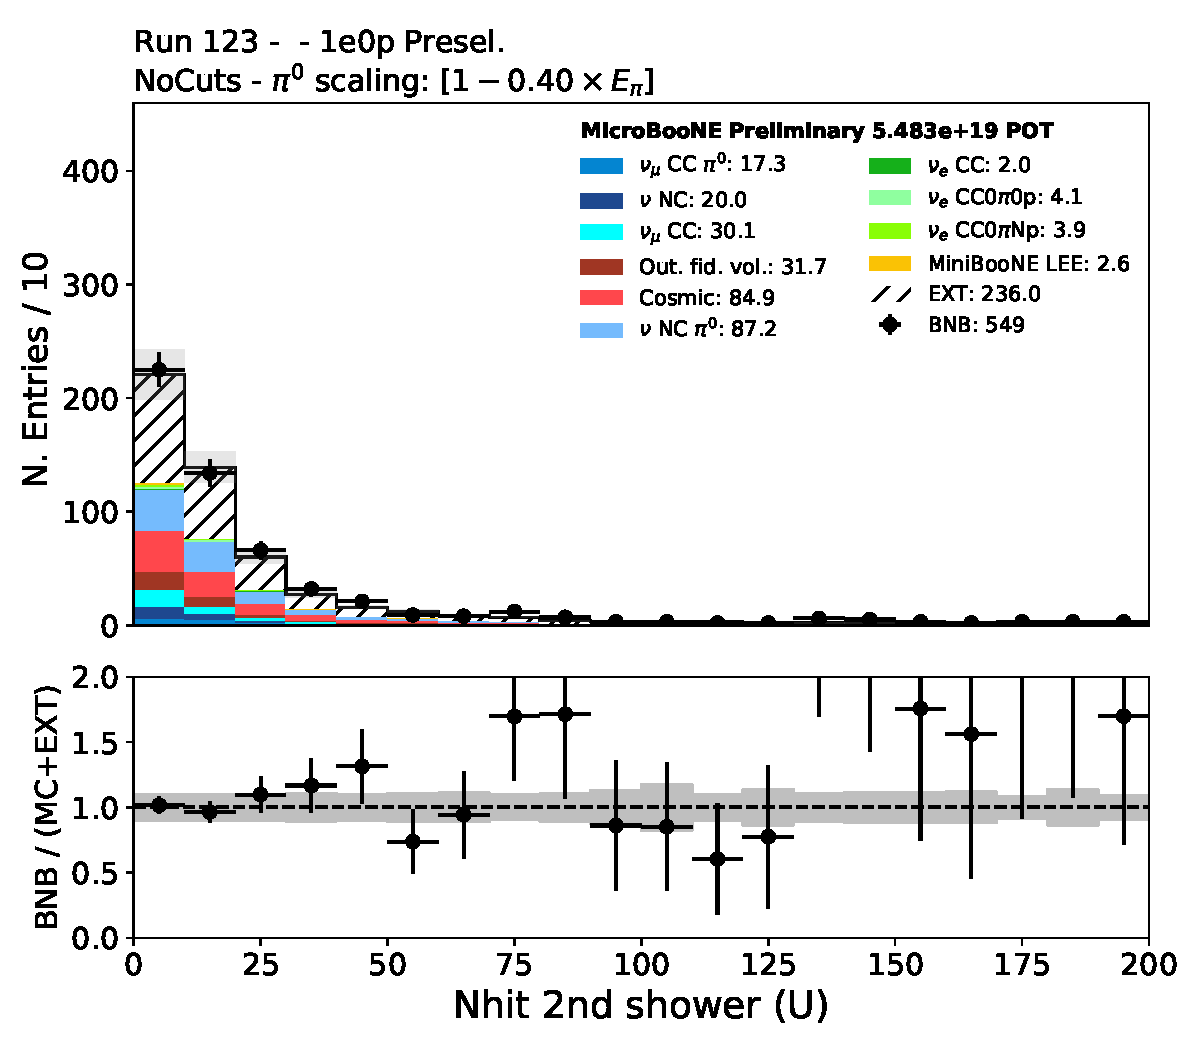
\includegraphics[width=1.00\textwidth]{1e0p/dataMCRun123/secondshower_U_nhit.pdf}
    \caption{\label{fig:1e0p:dataMCRun1:secondshower_U_nhit} secondshower\_U\_nhit }
    \end{subfigure}
\caption{\label{fig:1e0p:dataMCRun1:pi01}Data-MC comparison in the open data after the \zpsel preselection.}
\end{center}
\end{figure}

\begin{figure}[H] 
\begin{center}
    \begin{subfigure}[b]{0.3\textwidth}
    \centering
    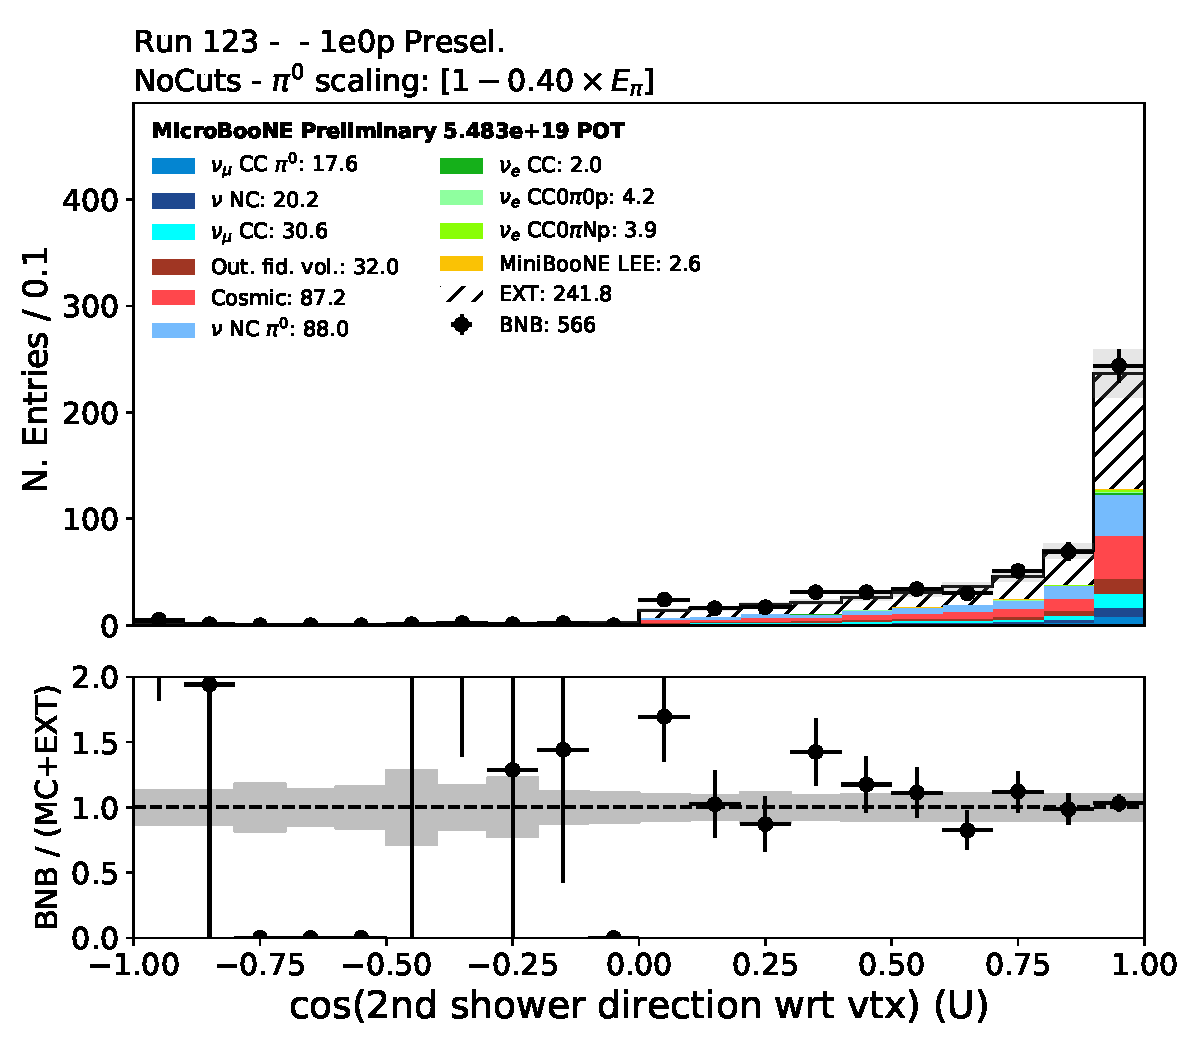
\includegraphics[width=1.00\textwidth]{1e0p/dataMCRun123/secondshower_U_dot.pdf}
    \caption{\label{fig:1e0p:dataMCRun1:secondshower_U_dot} secondshower\_U\_dot }
    \end{subfigure}
    \begin{subfigure}[b]{0.3\textwidth}
    \centering
    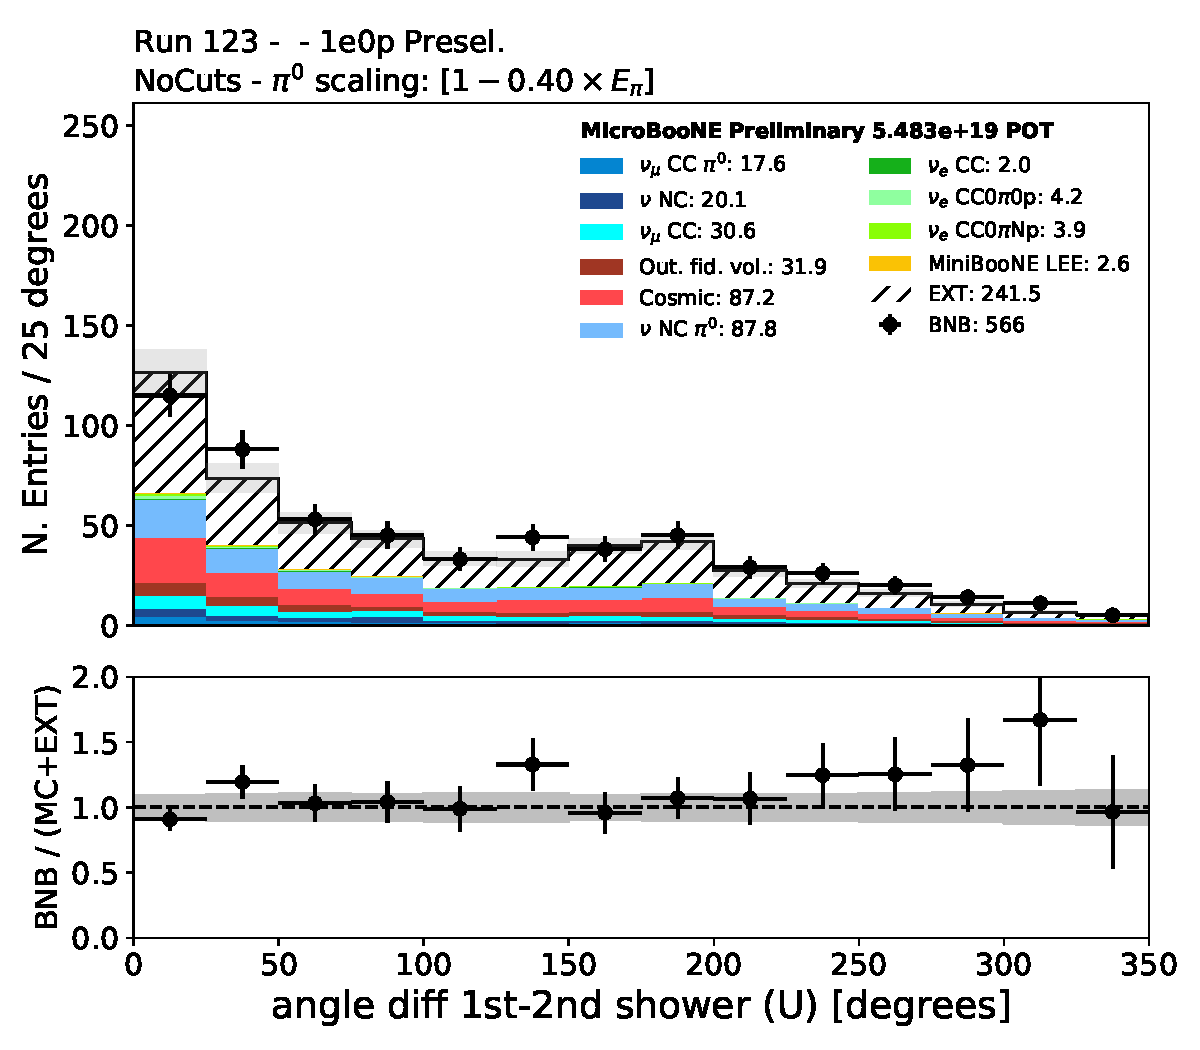
\includegraphics[width=1.00\textwidth]{1e0p/dataMCRun123/anglediff_U.pdf}
    \caption{\label{fig:1e0p:dataMCRun1:anglediff_U} anglediff\_U }
    \end{subfigure}
\caption{\label{fig:1e0p:dataMCRun1:pi02U}Data-MC comparison in the open data after the \zpsel preselection.}
\end{center}
\end{figure}

\begin{figure}[H] 
\begin{center}
    \begin{subfigure}[b]{0.3\textwidth}
    \centering
    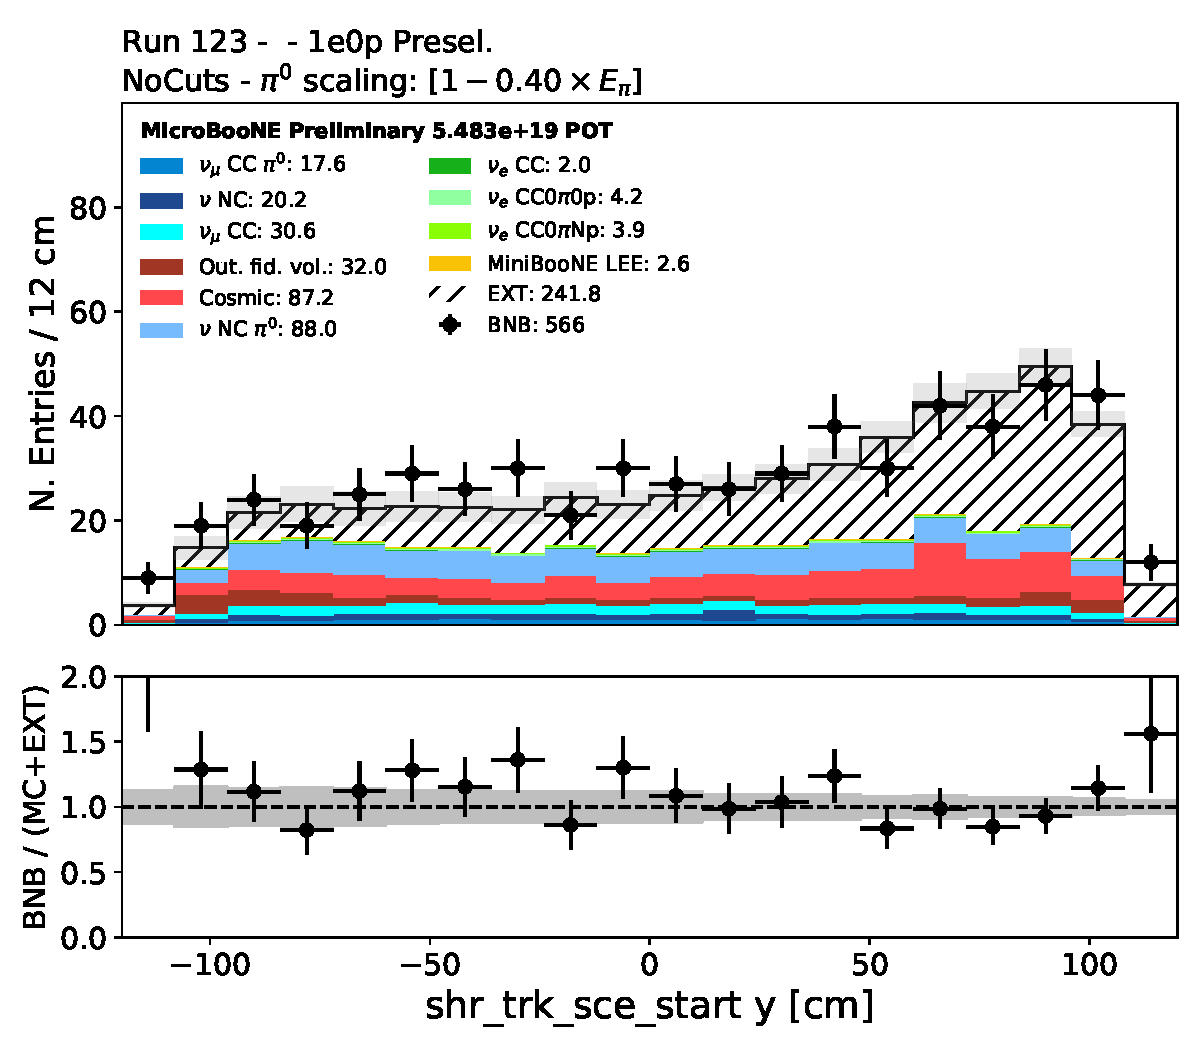
\includegraphics[width=1.00\textwidth]{1e0p/dataMCRun123/shr_trk_sce_start_y.pdf}
    \caption{\label{fig:1e0p:dataMCRun1:shr_start_y} shr\_trk\_sce\_start\_y }
    \end{subfigure}
    \begin{subfigure}[b]{0.3\textwidth}
    \centering
    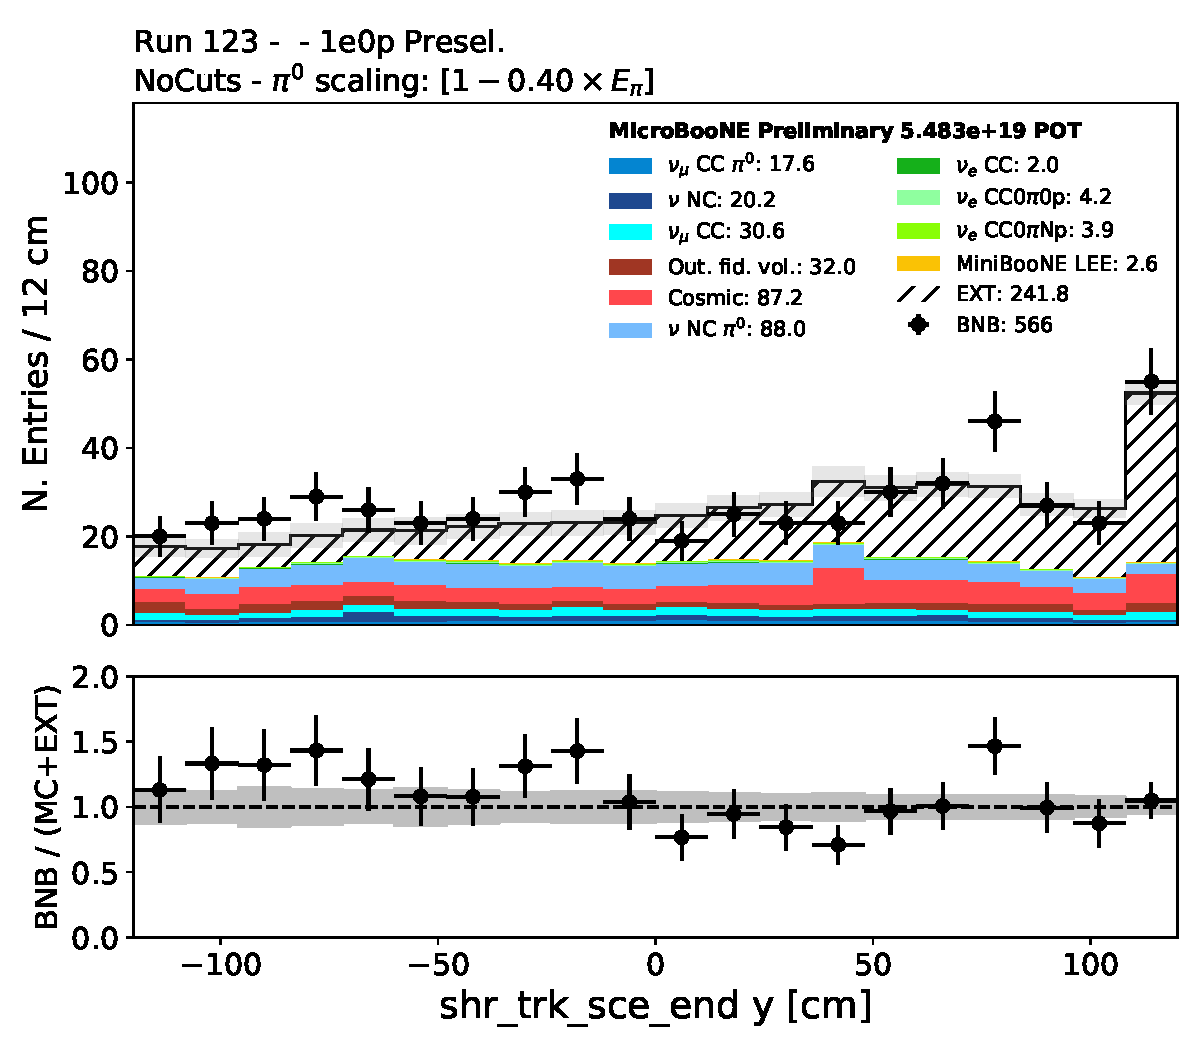
\includegraphics[width=1.00\textwidth]{1e0p/dataMCRun123/shr_trk_sce_end_y.pdf}
    \caption{\label{fig:1e0p:dataMCRun1:shr_end_y} shr\_trk\_sce\_end\_y }
    \end{subfigure}
\caption{\label{fig:1e0p:dataMCRun1:shrstartend}Data-MC comparison in the open data after the \zpsel preselection.}
\end{center}
\end{figure}

\begin{figure}[H] 
\begin{center}
    \begin{subfigure}[b]{0.3\textwidth}
    \centering
    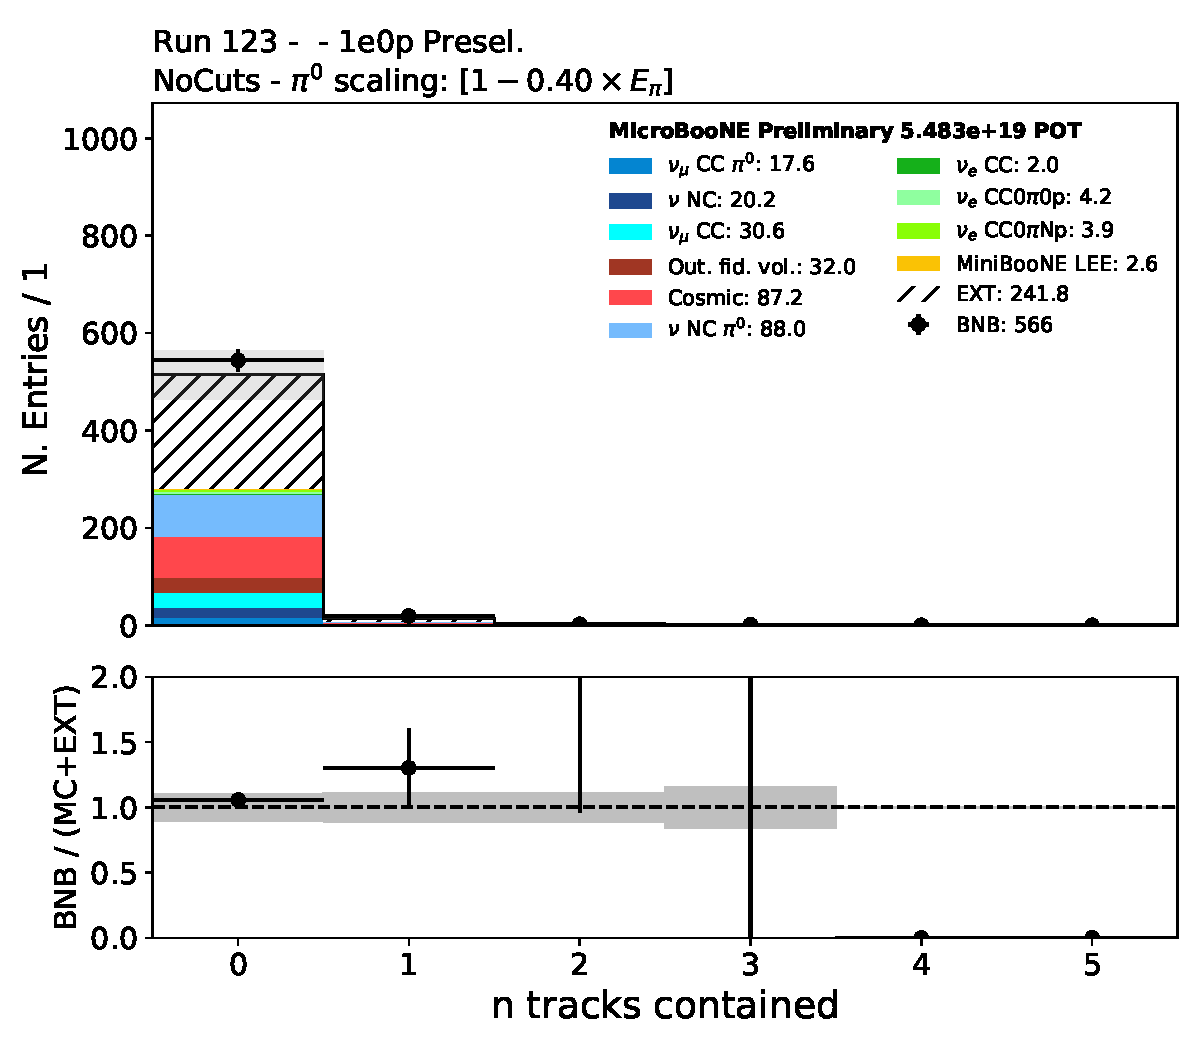
\includegraphics[width=1.00\textwidth]{1e0p/dataMCRun123/n_tracks_tot.pdf}
    \caption{\label{fig:1e0p:dataMCRun1:shr_start_y} n tracks tot }
    \end{subfigure}
    \begin{subfigure}[b]{0.3\textwidth}
    \centering
    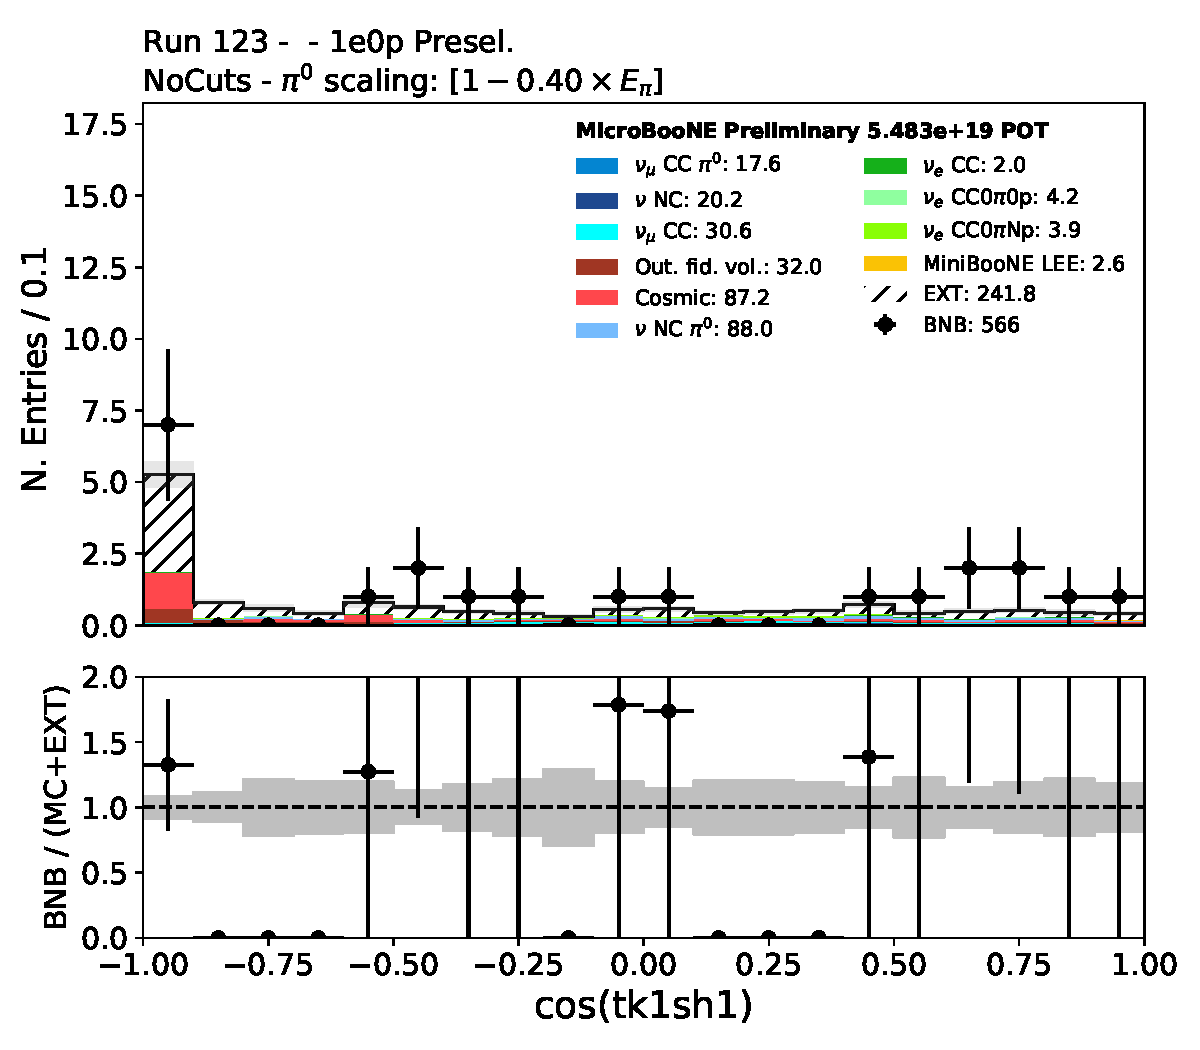
\includegraphics[width=1.00\textwidth]{1e0p/dataMCRun123/tk1sh1_angle_alltk.pdf}
    \caption{\label{fig:1e0p:dataMCRun1:shr_end_y} tk1 sh1 angle alltk }
    \end{subfigure}
\caption{\label{fig:1e0p:dataMCRun1:exitingtrack}Data-MC comparison in the open data after the \zpsel preselection.}
\end{center}
\end{figure}

\begin{figure}[H] 
\begin{center}
    \begin{subfigure}[b]{0.3\textwidth}
    \centering
    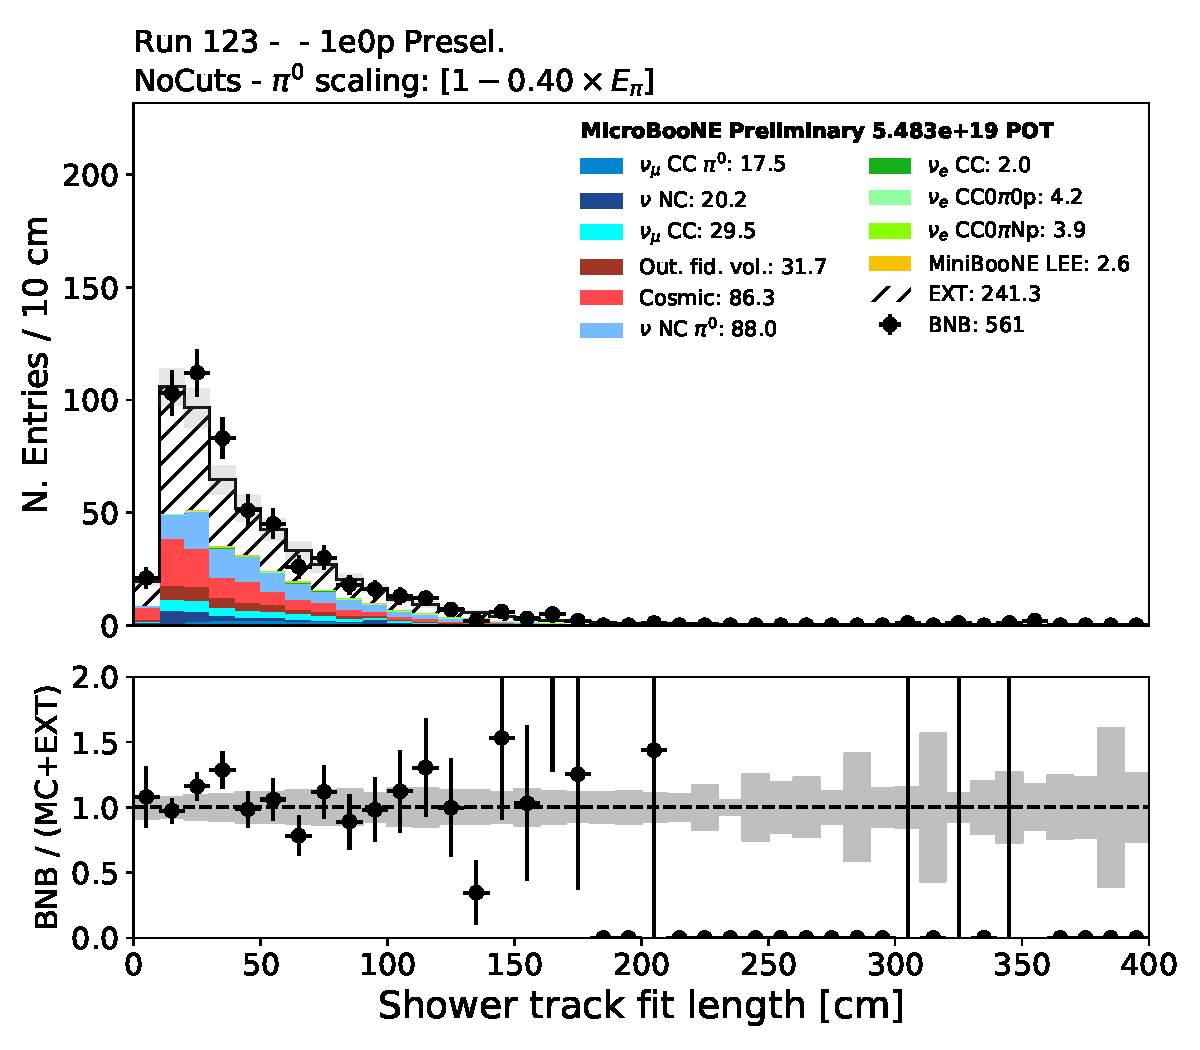
\includegraphics[width=1.00\textwidth]{1e0p/dataMCRun123/shr_trk_len.pdf}
    \caption{\label{fig:1e0p:dataMCRun1:shr_start_y} shr trk len }
    \end{subfigure}
    %\begin{subfigure}[b]{0.3\textwidth}
    %\centering
    %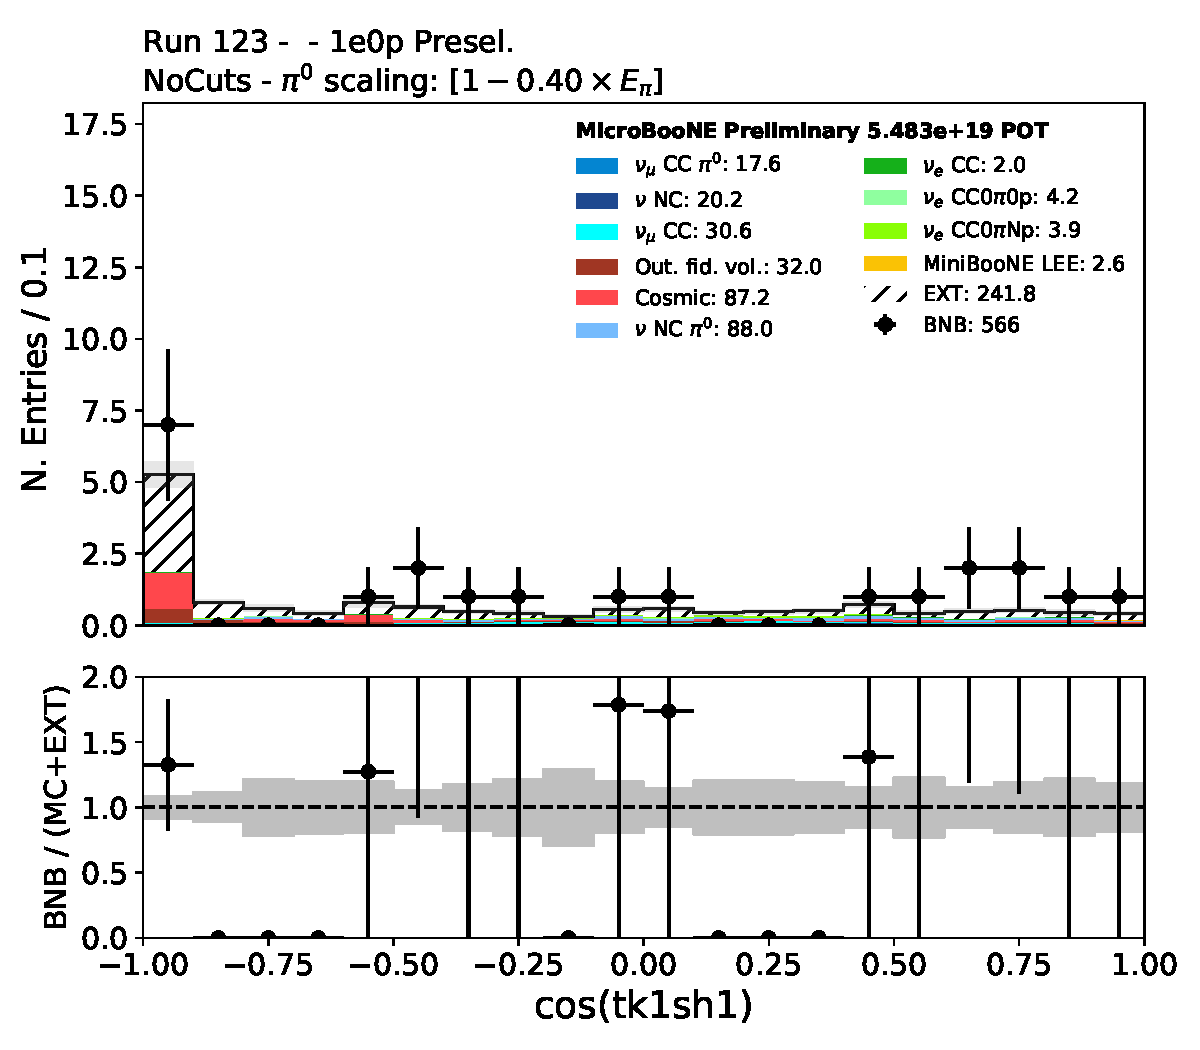
\includegraphics[width=1.00\textwidth]{1e0p/dataMCRun123/tk1sh1_angle_alltk.pdf}
   % \caption{\label{fig:1e0p:dataMCRun1:shr_end_y} tk1 sh1 angle alltk }
   % \end{subfigure}
\caption{\label{fig:1e0p:dataMCRun1:shrlen}Data-MC comparison in the open data after the \zpsel preselection.}
\end{center}
\end{figure}